\documentclass[1p]{elsarticle_modified}
%\bibliographystyle{elsarticle-num}

%\usepackage[colorlinks]{hyperref}
%\usepackage{abbrmath_seonhwa} %\Abb, \Ascr, \Acal ,\Abf, \Afrak
\usepackage{amsfonts}
\usepackage{amssymb}
\usepackage{amsmath}
\usepackage{amsthm}
\usepackage{scalefnt}
\usepackage{amsbsy}
\usepackage{kotex}
\usepackage{caption}
\usepackage{subfig}
\usepackage{color}
\usepackage{graphicx}
\usepackage{xcolor} %% white, black, red, green, blue, cyan, magenta, yellow
\usepackage{float}
\usepackage{setspace}
\usepackage{hyperref}

\usepackage{tikz}
\usetikzlibrary{arrows}

\usepackage{multirow}
\usepackage{array} % fixed length table
\usepackage{hhline}

%%%%%%%%%%%%%%%%%%%%%
\makeatletter
\renewcommand*\env@matrix[1][\arraystretch]{%
	\edef\arraystretch{#1}%
	\hskip -\arraycolsep
	\let\@ifnextchar\new@ifnextchar
	\array{*\c@MaxMatrixCols c}}
\makeatother %https://tex.stackexchange.com/questions/14071/how-can-i-increase-the-line-spacing-in-a-matrix
%%%%%%%%%%%%%%%

\usepackage[normalem]{ulem}

\newcommand{\msout}[1]{\ifmmode\text{\sout{\ensuremath{#1}}}\else\sout{#1}\fi}
%SOURCE: \msout is \stkout macro in https://tex.stackexchange.com/questions/20609/strikeout-in-math-mode

\newcommand{\cancel}[1]{
	\ifmmode
	{\color{red}\msout{#1}}
	\else
	{\color{red}\sout{#1}}
	\fi
}

\newcommand{\add}[1]{
	{\color{blue}\uwave{#1}}
}

\newcommand{\replace}[2]{
	\ifmmode
	{\color{red}\msout{#1}}{\color{blue}\uwave{#2}}
	\else
	{\color{red}\sout{#1}}{\color{blue}\uwave{#2}}
	\fi
}

\newcommand{\Sol}{\mathcal{S}} %segment
\newcommand{\D}{D} %diagram
\newcommand{\A}{\mathcal{A}} %arc


%%%%%%%%%%%%%%%%%%%%%%%%%%%%%5 test

\def\sl{\operatorname{\textup{SL}}(2,\Cbb)}
\def\psl{\operatorname{\textup{PSL}}(2,\Cbb)}
\def\quan{\mkern 1mu \triangleright \mkern 1mu}

\theoremstyle{definition}
\newtheorem{thm}{Theorem}[section]
\newtheorem{prop}[thm]{Proposition}
\newtheorem{lem}[thm]{Lemma}
\newtheorem{ques}[thm]{Question}
\newtheorem{cor}[thm]{Corollary}
\newtheorem{defn}[thm]{Definition}
\newtheorem{exam}[thm]{Example}
\newtheorem{rmk}[thm]{Remark}
\newtheorem{alg}[thm]{Algorithm}

\newcommand{\I}{\sqrt{-1}}
\begin{document}

%\begin{frontmatter}
%
%\title{Boundary parabolic representations of knots up to 8 crossings}
%
%%% Group authors per affiliation:
%\author{Yunhi Cho} 
%\address{Department of Mathematics, University of Seoul, Seoul, Korea}
%\ead{yhcho@uos.ac.kr}
%
%
%\author{Seonhwa Kim} %\fnref{s_kim}}
%\address{Center for Geometry and Physics, Institute for Basic Science, Pohang, 37673, Korea}
%\ead{ryeona17@ibs.re.kr}
%
%\author{Hyuk Kim}
%\address{Department of Mathematical Sciences, Seoul National University, Seoul 08826, Korea}
%\ead{hyukkim@snu.ac.kr}
%
%\author{Seokbeom Yoon}
%\address{Department of Mathematical Sciences, Seoul National University, Seoul, 08826,  Korea}
%\ead{sbyoon15@snu.ac.kr}
%
%\begin{abstract}
%We find all boundary parabolic representation of knots up to 8 crossings.
%
%\end{abstract}
%\begin{keyword}
%    \MSC[2010] 57M25 
%\end{keyword}
%
%\end{frontmatter}

%\linenumbers
%\tableofcontents
%
\newcommand\colored[1]{\textcolor{white}{\rule[-0.35ex]{0.8em}{1.4ex}}\kern-0.8em\color{red} #1}%
%\newcommand\colored[1]{\textcolor{white}{ #1}\kern-2.17ex	\textcolor{white}{ #1}\kern-1.81ex	\textcolor{white}{ #1}\kern-2.15ex\color{red}#1	}

{\Large $\underline{12a_{1054}~(K12a_{1054})}$}

\setlength{\tabcolsep}{10pt}
\renewcommand{\arraystretch}{1.6}
\vspace{1cm}\begin{tabular}{m{100pt}>{\centering\arraybackslash}m{274pt}}
\multirow{5}{120pt}{
	\centering
	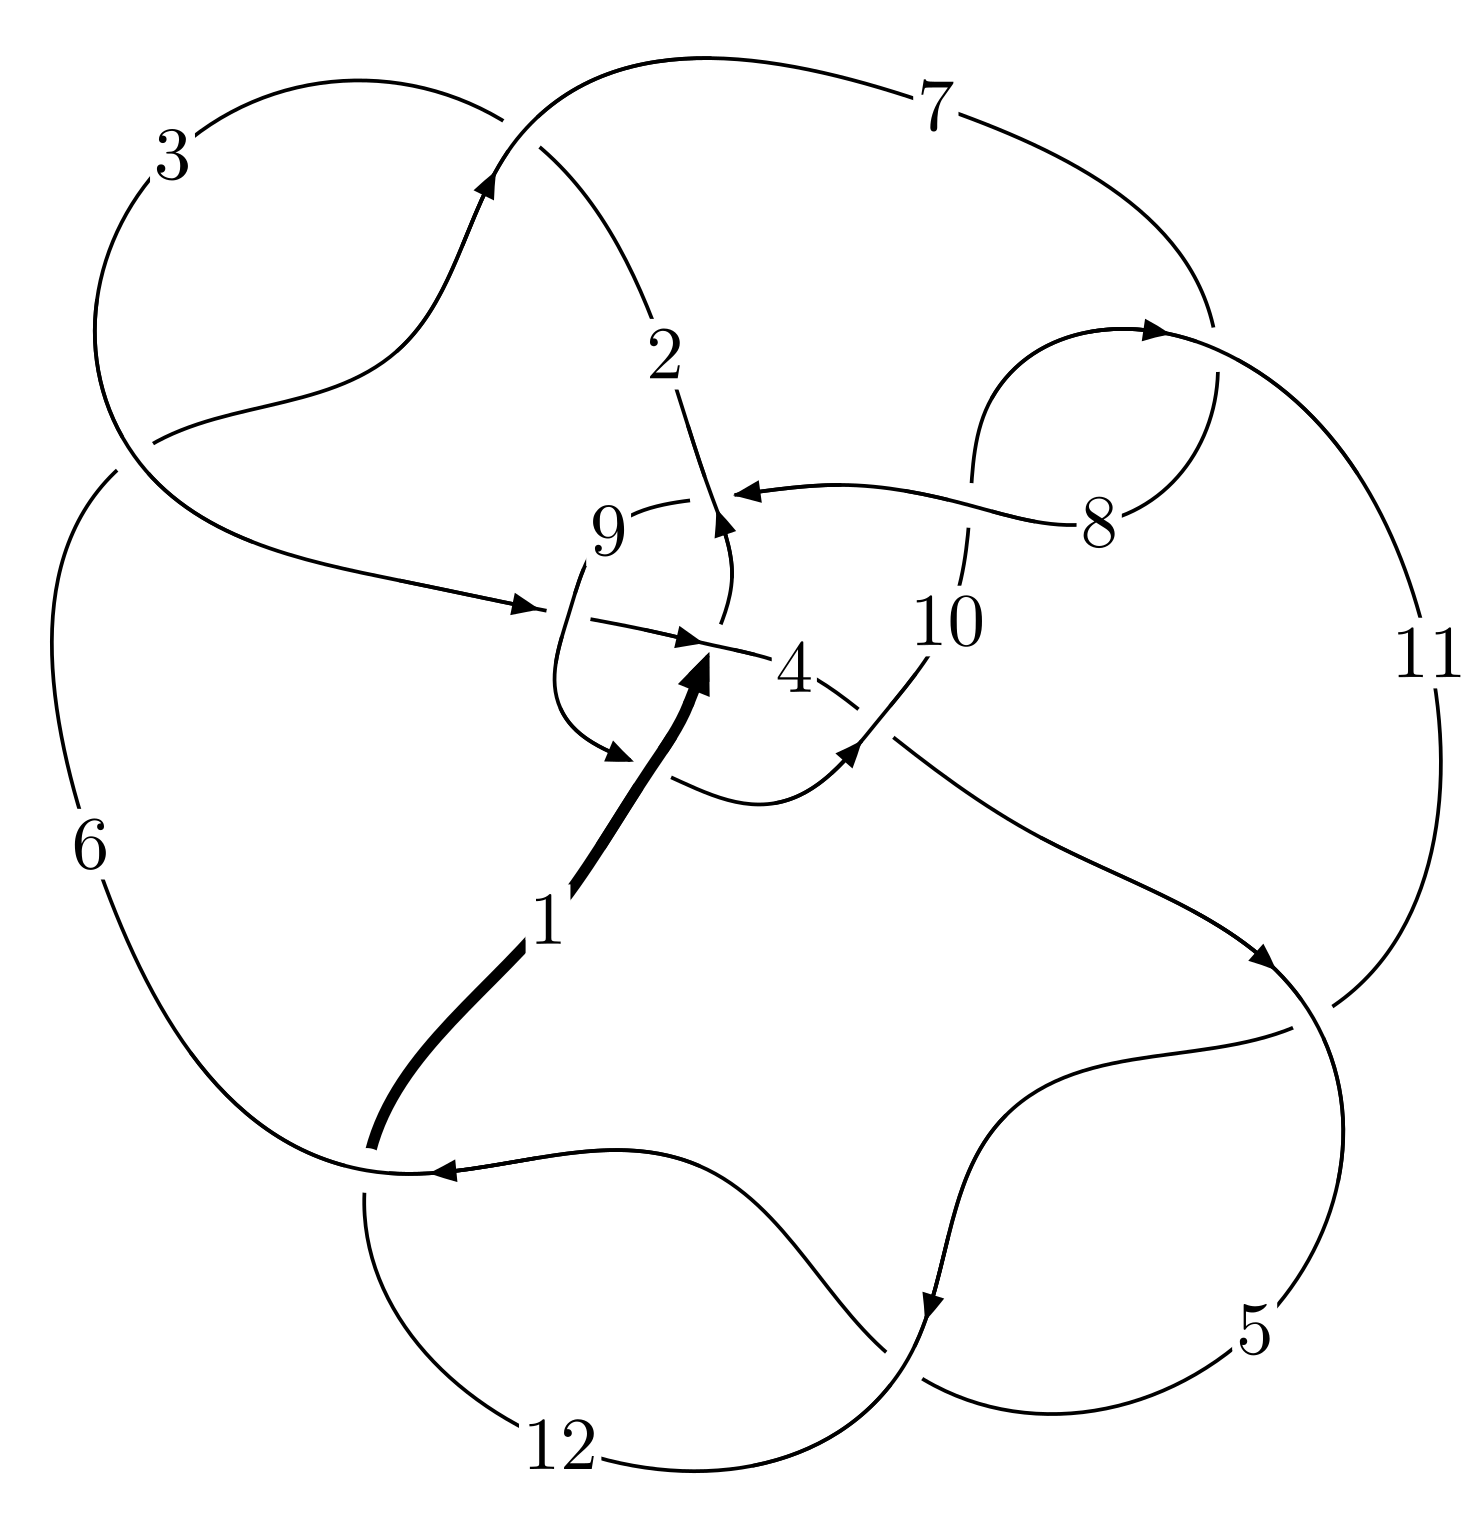
\includegraphics[width=112pt]{../../../GIT/diagram.site/Diagrams/png/1855_12a_1054.png}\\
\ \ \ A knot diagram\footnotemark}&
\allowdisplaybreaks
\textbf{Linearized knot diagam} \\
\cline{2-2}
 &
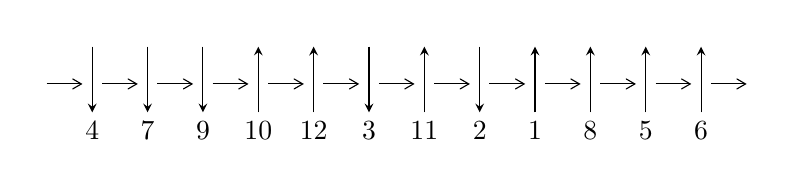
\begin{tikzpicture}[x=20pt, y=17pt]
	% nodes
	\node (C0) at (0, 0) {};
	\node (C1) at (1, 0) {};
	\node (C1U) at (1, +1) {};
	\node (C1D) at (1, -1) {4};

	\node (C2) at (2, 0) {};
	\node (C2U) at (2, +1) {};
	\node (C2D) at (2, -1) {7};

	\node (C3) at (3, 0) {};
	\node (C3U) at (3, +1) {};
	\node (C3D) at (3, -1) {9};

	\node (C4) at (4, 0) {};
	\node (C4U) at (4, +1) {};
	\node (C4D) at (4, -1) {10};

	\node (C5) at (5, 0) {};
	\node (C5U) at (5, +1) {};
	\node (C5D) at (5, -1) {12};

	\node (C6) at (6, 0) {};
	\node (C6U) at (6, +1) {};
	\node (C6D) at (6, -1) {3};

	\node (C7) at (7, 0) {};
	\node (C7U) at (7, +1) {};
	\node (C7D) at (7, -1) {11};

	\node (C8) at (8, 0) {};
	\node (C8U) at (8, +1) {};
	\node (C8D) at (8, -1) {2};

	\node (C9) at (9, 0) {};
	\node (C9U) at (9, +1) {};
	\node (C9D) at (9, -1) {1};

	\node (C10) at (10, 0) {};
	\node (C10U) at (10, +1) {};
	\node (C10D) at (10, -1) {8};

	\node (C11) at (11, 0) {};
	\node (C11U) at (11, +1) {};
	\node (C11D) at (11, -1) {5};

	\node (C12) at (12, 0) {};
	\node (C12U) at (12, +1) {};
	\node (C12D) at (12, -1) {6};
	\node (C13) at (13, 0) {};

	% arrows
	\draw[->,>={angle 60}]
	(C0) edge (C1) (C1) edge (C2) (C2) edge (C3) (C3) edge (C4) (C4) edge (C5) (C5) edge (C6) (C6) edge (C7) (C7) edge (C8) (C8) edge (C9) (C9) edge (C10) (C10) edge (C11) (C11) edge (C12) (C12) edge (C13) ;	\draw[->,>=stealth]
	(C1U) edge (C1D) (C2U) edge (C2D) (C3U) edge (C3D) (C4D) edge (C4U) (C5D) edge (C5U) (C6U) edge (C6D) (C7D) edge (C7U) (C8U) edge (C8D) (C9D) edge (C9U) (C10D) edge (C10U) (C11D) edge (C11U) (C12D) edge (C12U) ;
	\end{tikzpicture} \\
\hhline{~~} \\& 
\textbf{Solving Sequence} \\ \cline{2-2} 
 &
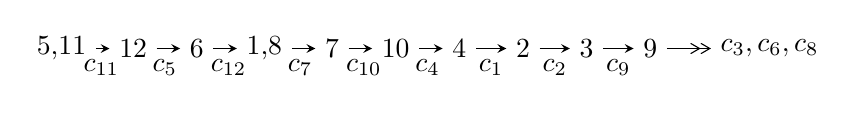
\begin{tikzpicture}[x=23pt, y=7pt]
	% node
	\node (A0) at (-1/8, 0) {5,11};
	\node (A1) at (1, 0) {12};
	\node (A2) at (2, 0) {6};
	\node (A3) at (49/16, 0) {1,8};
	\node (A4) at (33/8, 0) {7};
	\node (A5) at (41/8, 0) {10};
	\node (A6) at (49/8, 0) {4};
	\node (A7) at (57/8, 0) {2};
	\node (A8) at (65/8, 0) {3};
	\node (A9) at (73/8, 0) {9};
	\node (C1) at (1/2, -1) {$c_{11}$};
	\node (C2) at (3/2, -1) {$c_{5}$};
	\node (C3) at (5/2, -1) {$c_{12}$};
	\node (C4) at (29/8, -1) {$c_{7}$};
	\node (C5) at (37/8, -1) {$c_{10}$};
	\node (C6) at (45/8, -1) {$c_{4}$};
	\node (C7) at (53/8, -1) {$c_{1}$};
	\node (C8) at (61/8, -1) {$c_{2}$};
	\node (C9) at (69/8, -1) {$c_{9}$};
	\node (A10) at (11, 0) {$c_{3},c_{6},c_{8}$};

	% edge
	\draw[->,>=stealth]	
	(A0) edge (A1) (A1) edge (A2) (A2) edge (A3) (A3) edge (A4) (A4) edge (A5) (A5) edge (A6) (A6) edge (A7) (A7) edge (A8) (A8) edge (A9) ;
	\draw[->>,>={angle 60}]	
	(A9) edge (A10);
\end{tikzpicture} \\ 

\end{tabular} \\

\footnotetext{
The image of knot diagram is generated by the software ``\textbf{Draw programme}" developed by Andrew Bartholomew(\url{http://www.layer8.co.uk/maths/draw/index.htm\#Running-draw}), where we modified some parts for our purpose(\url{https://github.com/CATsTAILs/LinksPainter}).
}\phantom \\ \newline 
\centering \textbf{Ideals for irreducible components\footnotemark of $X_{\text{par}}$} 
 
\begin{align*}
I^u_{1}&=\langle 
2.15321\times10^{634} u^{158}-5.10063\times10^{634} u^{157}+\cdots+7.40198\times10^{634} b-2.87813\times10^{636},\\
\phantom{I^u_{1}}&\phantom{= \langle  }-1.60326\times10^{635} u^{158}+4.19807\times10^{635} u^{157}+\cdots+1.29871\times10^{636} a+3.54875\times10^{637},\\
\phantom{I^u_{1}}&\phantom{= \langle  }u^{159}- u^{158}+\cdots-2628 u-193\rangle \\
I^u_{2}&=\langle 
-3.16298\times10^{25} u^{45}-2.36685\times10^{25} u^{44}+\cdots+1.74991\times10^{25} b-3.55828\times10^{26},\\
\phantom{I^u_{2}}&\phantom{= \langle  }4.06958\times10^{26} u^{45}+3.57978\times10^{26} u^{44}+\cdots+5.24973\times10^{25} a+1.16350\times10^{27},\;u^{46}+2 u^{45}+\cdots+7 u+3\rangle \\
\\
\end{align*}
\raggedright * 2 irreducible components of $\dim_{\mathbb{C}}=0$, with total 205 representations.\\
\footnotetext{All coefficients of polynomials are rational numbers. But the coefficients are sometimes approximated in decimal forms when there is not enough margin.}
\newpage
\renewcommand{\arraystretch}{1}
\centering \section*{I. $I^u_{1}= \langle 2.15\times10^{634} u^{158}-5.10\times10^{634} u^{157}+\cdots+7.40\times10^{634} b-2.88\times10^{636},\;-1.60\times10^{635} u^{158}+4.20\times10^{635} u^{157}+\cdots+1.30\times10^{636} a+3.55\times10^{637},\;u^{159}- u^{158}+\cdots-2628 u-193 \rangle$}
\flushleft \textbf{(i) Arc colorings}\\
\begin{tabular}{m{7pt} m{180pt} m{7pt} m{180pt} }
\flushright $a_{5}=$&$\begin{pmatrix}0\\u\end{pmatrix}$ \\
\flushright $a_{11}=$&$\begin{pmatrix}1\\0\end{pmatrix}$ \\
\flushright $a_{12}=$&$\begin{pmatrix}1\\- u^2\end{pmatrix}$ \\
\flushright $a_{6}=$&$\begin{pmatrix}u\\- u^3+u\end{pmatrix}$ \\
\flushright $a_{1}=$&$\begin{pmatrix}- u^2+1\\u^4-2 u^2\end{pmatrix}$ \\
\flushright $a_{8}=$&$\begin{pmatrix}0.123450 u^{158}-0.323249 u^{157}+\cdots-307.540 u-27.3251\\-0.290897 u^{158}+0.689091 u^{157}+\cdots+483.939 u+38.8833\end{pmatrix}$ \\
\flushright $a_{7}=$&$\begin{pmatrix}0.414347 u^{158}-1.01234 u^{157}+\cdots-791.479 u-66.2084\\-0.290897 u^{158}+0.689091 u^{157}+\cdots+483.939 u+38.8833\end{pmatrix}$ \\
\flushright $a_{10}=$&$\begin{pmatrix}-1.09858 u^{158}+2.52398 u^{157}+\cdots+1949.19 u+151.364\\1.01751 u^{158}-2.21497 u^{157}+\cdots-2093.91 u-162.844\end{pmatrix}$ \\
\flushright $a_{4}=$&$\begin{pmatrix}-2.82070 u^{158}+6.50241 u^{157}+\cdots+5629.10 u+439.227\\-0.470943 u^{158}+1.22959 u^{157}+\cdots+686.317 u+52.3871\end{pmatrix}$ \\
\flushright $a_{2}=$&$\begin{pmatrix}0.458496 u^{158}-1.13570 u^{157}+\cdots-955.257 u-72.1383\\-0.287925 u^{158}+0.710940 u^{157}+\cdots+443.599 u+32.8072\end{pmatrix}$ \\
\flushright $a_{3}=$&$\begin{pmatrix}0.828370 u^{158}-2.00213 u^{157}+\cdots-1693.31 u-130.632\\-0.485796 u^{158}+1.14028 u^{157}+\cdots+910.425 u+69.5863\end{pmatrix}$ \\
\flushright $a_{9}=$&$\begin{pmatrix}-1.51656 u^{158}+3.41746 u^{157}+\cdots+2800.47 u+217.244\\0.135899 u^{158}-0.219030 u^{157}+\cdots-365.250 u-27.9326\end{pmatrix}$\\&\end{tabular}
\flushleft \textbf{(ii) Obstruction class $= -1$}\\~\\
\flushleft \textbf{(iii) Cusp Shapes $= -5.99897 u^{158}+12.6571 u^{157}+\cdots+12926.8 u+1026.83$}\\~\\
\newpage\renewcommand{\arraystretch}{1}
\flushleft \textbf{(iv) u-Polynomials at the component}\newline \\
\begin{tabular}{m{50pt}|m{274pt}}
Crossings & \hspace{64pt}u-Polynomials at each crossing \\
\hline $$\begin{aligned}c_{1}\end{aligned}$$&$\begin{aligned}
&u^{159}-11 u^{158}+\cdots-43 u+11
\end{aligned}$\\
\hline $$\begin{aligned}c_{2},c_{6}\end{aligned}$$&$\begin{aligned}
&u^{159}-3 u^{158}+\cdots-71881 u-10679
\end{aligned}$\\
\hline $$\begin{aligned}c_{3}\end{aligned}$$&$\begin{aligned}
&u^{159}+u^{158}+\cdots+527 u-25
\end{aligned}$\\
\hline $$\begin{aligned}c_{4}\end{aligned}$$&$\begin{aligned}
&u^{159}- u^{158}+\cdots+46182518 u-10020811
\end{aligned}$\\
\hline $$\begin{aligned}c_{5},c_{11},c_{12}\end{aligned}$$&$\begin{aligned}
&u^{159}- u^{158}+\cdots-2628 u-193
\end{aligned}$\\
\hline $$\begin{aligned}c_{7},c_{10}\end{aligned}$$&$\begin{aligned}
&u^{159}-12 u^{158}+\cdots+53726 u+16181
\end{aligned}$\\
\hline $$\begin{aligned}c_{8}\end{aligned}$$&$\begin{aligned}
&u^{159}- u^{158}+\cdots-8791546 u-1048243
\end{aligned}$\\
\hline $$\begin{aligned}c_{9}\end{aligned}$$&$\begin{aligned}
&u^{159}-5 u^{158}+\cdots-16779 u+1957
\end{aligned}$\\
\hline
\end{tabular}\\~\\
\newpage\renewcommand{\arraystretch}{1}
\flushleft \textbf{(v) Riley Polynomials at the component}\newline \\
\begin{tabular}{m{50pt}|m{274pt}}
Crossings & \hspace{64pt}Riley Polynomials at each crossing \\
\hline $$\begin{aligned}c_{1}\end{aligned}$$&$\begin{aligned}
&y^{159}+7 y^{158}+\cdots-6709 y-121
\end{aligned}$\\
\hline $$\begin{aligned}c_{2},c_{6}\end{aligned}$$&$\begin{aligned}
&y^{159}+97 y^{158}+\cdots-5702976927 y-114041041
\end{aligned}$\\
\hline $$\begin{aligned}c_{3}\end{aligned}$$&$\begin{aligned}
&y^{159}+17 y^{158}+\cdots-58921 y-625
\end{aligned}$\\
\hline $$\begin{aligned}c_{4}\end{aligned}$$&$\begin{aligned}
&y^{159}-15 y^{158}+\cdots+1162437248935440 y-100416653097721
\end{aligned}$\\
\hline $$\begin{aligned}c_{5},c_{11},c_{12}\end{aligned}$$&$\begin{aligned}
&y^{159}-159 y^{158}+\cdots-2425166 y-37249
\end{aligned}$\\
\hline $$\begin{aligned}c_{7},c_{10}\end{aligned}$$&$\begin{aligned}
&y^{159}+70 y^{158}+\cdots-10616690872 y-261824761
\end{aligned}$\\
\hline $$\begin{aligned}c_{8}\end{aligned}$$&$\begin{aligned}
&y^{159}+11 y^{158}+\cdots-57826335947932 y-1098813387049
\end{aligned}$\\
\hline $$\begin{aligned}c_{9}\end{aligned}$$&$\begin{aligned}
&y^{159}-21 y^{158}+\cdots+100453631 y-3829849
\end{aligned}$\\
\hline
\end{tabular}\\~\\
\newpage\flushleft \textbf{(vi) Complex Volumes and Cusp Shapes}
$$\begin{array}{c|c|c}  
\text{Solutions to }I^u_{1}& \I (\text{vol} + \sqrt{-1}CS) & \text{Cusp shape}\\
 \hline 
\begin{aligned}
u &= -0.931695 + 0.357791 I \\
a &= -0.97351 - 1.30496 I \\
b &= \phantom{-}0.004696 - 0.961026 I\end{aligned}
 & -3.10088 - 3.11572 I & \phantom{-0.000000 } 0 \\ \hline\begin{aligned}
u &= -0.931695 - 0.357791 I \\
a &= -0.97351 + 1.30496 I \\
b &= \phantom{-}0.004696 + 0.961026 I\end{aligned}
 & -3.10088 + 3.11572 I & \phantom{-0.000000 } 0 \\ \hline\begin{aligned}
u &= \phantom{-}0.168571 + 0.972045 I \\
a &= \phantom{-}0.26892 + 1.60345 I \\
b &= \phantom{-}0.250633 + 1.204880 I\end{aligned}
 & -2.82090 + 2.76288 I & \phantom{-0.000000 } 0 \\ \hline\begin{aligned}
u &= \phantom{-}0.168571 - 0.972045 I \\
a &= \phantom{-}0.26892 - 1.60345 I \\
b &= \phantom{-}0.250633 - 1.204880 I\end{aligned}
 & -2.82090 - 2.76288 I & \phantom{-0.000000 } 0 \\ \hline\begin{aligned}
u &= \phantom{-}0.458881 + 0.956536 I \\
a &= \phantom{-}0.31707 - 1.71133 I \\
b &= -0.664222 - 1.214920 I\end{aligned}
 & \phantom{-}0.9763 + 15.2232 I & \phantom{-0.000000 } 0 \\ \hline\begin{aligned}
u &= \phantom{-}0.458881 - 0.956536 I \\
a &= \phantom{-}0.31707 + 1.71133 I \\
b &= -0.664222 + 1.214920 I\end{aligned}
 & \phantom{-}0.9763 - 15.2232 I & \phantom{-0.000000 } 0 \\ \hline\begin{aligned}
u &= \phantom{-}0.639690 + 0.887084 I \\
a &= \phantom{-}0.185987 + 0.895267 I \\
b &= -0.489570 + 0.646391 I\end{aligned}
 & \phantom{-}1.65184 + 1.81096 I & \phantom{-0.000000 } 0 \\ \hline\begin{aligned}
u &= \phantom{-}0.639690 - 0.887084 I \\
a &= \phantom{-}0.185987 - 0.895267 I \\
b &= -0.489570 - 0.646391 I\end{aligned}
 & \phantom{-}1.65184 - 1.81096 I & \phantom{-0.000000 } 0 \\ \hline\begin{aligned}
u &= -0.528201 + 0.999238 I \\
a &= -0.19425 - 1.59774 I \\
b &= \phantom{-}0.388374 - 1.012770 I\end{aligned}
 & -1.51699 - 4.68944 I & \phantom{-0.000000 } 0 \\ \hline\begin{aligned}
u &= -0.528201 - 0.999238 I \\
a &= -0.19425 + 1.59774 I \\
b &= \phantom{-}0.388374 + 1.012770 I\end{aligned}
 & -1.51699 + 4.68944 I & \phantom{-0.000000 } 0\\
 \hline 
 \end{array}$$\newpage$$\begin{array}{c|c|c}  
\text{Solutions to }I^u_{1}& \I (\text{vol} + \sqrt{-1}CS) & \text{Cusp shape}\\
 \hline 
\begin{aligned}
u &= \phantom{-}0.638750 + 0.582865 I \\
a &= \phantom{-}0.814828 + 0.739374 I \\
b &= -0.289334 + 0.388871 I\end{aligned}
 & \phantom{-}1.56860 + 1.91000 I & \phantom{-0.000000 } 0 \\ \hline\begin{aligned}
u &= \phantom{-}0.638750 - 0.582865 I \\
a &= \phantom{-}0.814828 - 0.739374 I \\
b &= -0.289334 - 0.388871 I\end{aligned}
 & \phantom{-}1.56860 - 1.91000 I & \phantom{-0.000000 } 0 \\ \hline\begin{aligned}
u &= -0.721937 + 0.473511 I \\
a &= -0.455318 - 1.317190 I \\
b &= \phantom{-}0.581524 - 1.284450 I\end{aligned}
 & \phantom{-}0.48072 - 6.90966 I & \phantom{-0.000000 } 0 \\ \hline\begin{aligned}
u &= -0.721937 - 0.473511 I \\
a &= -0.455318 + 1.317190 I \\
b &= \phantom{-}0.581524 + 1.284450 I\end{aligned}
 & \phantom{-}0.48072 + 6.90966 I & \phantom{-0.000000 } 0 \\ \hline\begin{aligned}
u &= \phantom{-}0.414790 + 0.756611 I \\
a &= -0.472518 + 0.338296 I \\
b &= -1.066210 + 0.353597 I\end{aligned}
 & \phantom{-}3.66257 + 9.07043 I & \phantom{-0.000000 } 0 \\ \hline\begin{aligned}
u &= \phantom{-}0.414790 - 0.756611 I \\
a &= -0.472518 - 0.338296 I \\
b &= -1.066210 - 0.353597 I\end{aligned}
 & \phantom{-}3.66257 - 9.07043 I & \phantom{-0.000000 } 0 \\ \hline\begin{aligned}
u &= \phantom{-}0.956897 + 0.615982 I \\
a &= -0.089603 + 0.314750 I \\
b &= -0.529731 + 0.880357 I\end{aligned}
 & \phantom{-}2.75523 - 0.19630 I & \phantom{-0.000000 } 0 \\ \hline\begin{aligned}
u &= \phantom{-}0.956897 - 0.615982 I \\
a &= -0.089603 - 0.314750 I \\
b &= -0.529731 - 0.880357 I\end{aligned}
 & \phantom{-}2.75523 + 0.19630 I & \phantom{-0.000000 } 0 \\ \hline\begin{aligned}
u &= -0.411723 + 0.748664 I \\
a &= \phantom{-}0.43991 + 2.19502 I \\
b &= -0.515799 + 1.108660 I\end{aligned}
 & -2.52177 - 9.07559 I & \phantom{-0.000000 } 0 \\ \hline\begin{aligned}
u &= -0.411723 - 0.748664 I \\
a &= \phantom{-}0.43991 - 2.19502 I \\
b &= -0.515799 - 1.108660 I\end{aligned}
 & -2.52177 + 9.07559 I & \phantom{-0.000000 } 0\\
 \hline 
 \end{array}$$\newpage$$\begin{array}{c|c|c}  
\text{Solutions to }I^u_{1}& \I (\text{vol} + \sqrt{-1}CS) & \text{Cusp shape}\\
 \hline 
\begin{aligned}
u &= \phantom{-}0.400836 + 1.077030 I \\
a &= \phantom{-}0.37746 - 1.40274 I \\
b &= -0.564630 - 0.986860 I\end{aligned}
 & \phantom{-}0.56231 + 6.26018 I & \phantom{-0.000000 } 0 \\ \hline\begin{aligned}
u &= \phantom{-}0.400836 - 1.077030 I \\
a &= \phantom{-}0.37746 + 1.40274 I \\
b &= -0.564630 + 0.986860 I\end{aligned}
 & \phantom{-}0.56231 - 6.26018 I & \phantom{-0.000000 } 0 \\ \hline\begin{aligned}
u &= \phantom{-}0.564617 + 0.634758 I \\
a &= \phantom{-}0.52541 - 1.89259 I \\
b &= -0.595660 - 0.351204 I\end{aligned}
 & \phantom{-}4.28308 - 4.47208 I & \phantom{-0.000000 } 0 \\ \hline\begin{aligned}
u &= \phantom{-}0.564617 - 0.634758 I \\
a &= \phantom{-}0.52541 + 1.89259 I \\
b &= -0.595660 + 0.351204 I\end{aligned}
 & \phantom{-}4.28308 + 4.47208 I & \phantom{-0.000000 } 0 \\ \hline\begin{aligned}
u &= \phantom{-}1.162030 + 0.179115 I \\
a &= \phantom{-}1.067080 - 0.683283 I \\
b &= \phantom{-}0.029357 - 0.888191 I\end{aligned}
 & \phantom{-}1.055130 + 0.194599 I & \phantom{-0.000000 } 0 \\ \hline\begin{aligned}
u &= \phantom{-}1.162030 - 0.179115 I \\
a &= \phantom{-}1.067080 + 0.683283 I \\
b &= \phantom{-}0.029357 + 0.888191 I\end{aligned}
 & \phantom{-}1.055130 - 0.194599 I & \phantom{-0.000000 } 0 \\ \hline\begin{aligned}
u &= -1.153970 + 0.230467 I \\
a &= \phantom{-}0.045014 - 0.836283 I \\
b &= \phantom{-}0.201484 - 1.114320 I\end{aligned}
 & \phantom{-}1.80742 - 4.76661 I & \phantom{-0.000000 } 0 \\ \hline\begin{aligned}
u &= -1.153970 - 0.230467 I \\
a &= \phantom{-}0.045014 + 0.836283 I \\
b &= \phantom{-}0.201484 + 1.114320 I\end{aligned}
 & \phantom{-}1.80742 + 4.76661 I & \phantom{-0.000000 } 0 \\ \hline\begin{aligned}
u &= \phantom{-}1.030560 + 0.574716 I \\
a &= \phantom{-}1.21600 - 1.14196 I \\
b &= -0.620859 - 0.793677 I\end{aligned}
 & \phantom{-}3.09533 + 4.35647 I & \phantom{-0.000000 } 0 \\ \hline\begin{aligned}
u &= \phantom{-}1.030560 - 0.574716 I \\
a &= \phantom{-}1.21600 + 1.14196 I \\
b &= -0.620859 + 0.793677 I\end{aligned}
 & \phantom{-}3.09533 - 4.35647 I & \phantom{-0.000000 } 0\\
 \hline 
 \end{array}$$\newpage$$\begin{array}{c|c|c}  
\text{Solutions to }I^u_{1}& \I (\text{vol} + \sqrt{-1}CS) & \text{Cusp shape}\\
 \hline 
\begin{aligned}
u &= -0.722581 + 0.380203 I \\
a &= -1.03917 - 1.19458 I \\
b &= -0.400454 - 0.823490 I\end{aligned}
 & -1.63826 + 4.76979 I & \phantom{-0.000000 } 0 \\ \hline\begin{aligned}
u &= -0.722581 - 0.380203 I \\
a &= -1.03917 + 1.19458 I \\
b &= -0.400454 + 0.823490 I\end{aligned}
 & -1.63826 - 4.76979 I & \phantom{-0.000000 } 0 \\ \hline\begin{aligned}
u &= -0.136279 + 0.782606 I \\
a &= \phantom{-}0.312504 + 1.346250 I \\
b &= -0.318155 + 0.828940 I\end{aligned}
 & -1.31506 + 1.03769 I & \phantom{-0.000000 } 0 \\ \hline\begin{aligned}
u &= -0.136279 - 0.782606 I \\
a &= \phantom{-}0.312504 - 1.346250 I \\
b &= -0.318155 - 0.828940 I\end{aligned}
 & -1.31506 - 1.03769 I & \phantom{-0.000000 } 0 \\ \hline\begin{aligned}
u &= \phantom{-}0.850317 + 0.864003 I \\
a &= -0.518250 + 0.783787 I \\
b &= -0.549421 + 1.113070 I\end{aligned}
 & \phantom{-}2.05790 - 9.12170 I & \phantom{-0.000000 } 0 \\ \hline\begin{aligned}
u &= \phantom{-}0.850317 - 0.864003 I \\
a &= -0.518250 - 0.783787 I \\
b &= -0.549421 - 1.113070 I\end{aligned}
 & \phantom{-}2.05790 + 9.12170 I & \phantom{-0.000000 } 0 \\ \hline\begin{aligned}
u &= -1.210660 + 0.081806 I \\
a &= -0.24605 - 1.62594 I \\
b &= \phantom{-}0.42389 - 1.37878 I\end{aligned}
 & \phantom{-}0.86122 - 6.29681 I & \phantom{-0.000000 } 0 \\ \hline\begin{aligned}
u &= -1.210660 - 0.081806 I \\
a &= -0.24605 + 1.62594 I \\
b &= \phantom{-}0.42389 + 1.37878 I\end{aligned}
 & \phantom{-}0.86122 + 6.29681 I & \phantom{-0.000000 } 0 \\ \hline\begin{aligned}
u &= \phantom{-}0.454232 + 0.625845 I \\
a &= \phantom{-}1.44301 - 0.82043 I \\
b &= \phantom{-}0.121314 - 0.823882 I\end{aligned}
 & -0.600113 + 1.209260 I & \phantom{-0.000000 } 0 \\ \hline\begin{aligned}
u &= \phantom{-}0.454232 - 0.625845 I \\
a &= \phantom{-}1.44301 + 0.82043 I \\
b &= \phantom{-}0.121314 + 0.823882 I\end{aligned}
 & -0.600113 - 1.209260 I & \phantom{-0.000000 } 0\\
 \hline 
 \end{array}$$\newpage$$\begin{array}{c|c|c}  
\text{Solutions to }I^u_{1}& \I (\text{vol} + \sqrt{-1}CS) & \text{Cusp shape}\\
 \hline 
\begin{aligned}
u &= -0.371163 + 0.677094 I \\
a &= \phantom{-}0.947785 + 1.026760 I \\
b &= \phantom{-}0.671300 + 1.092560 I\end{aligned}
 & \phantom{-}1.42108 + 2.82655 I & \phantom{-0.000000 } 0 \\ \hline\begin{aligned}
u &= -0.371163 - 0.677094 I \\
a &= \phantom{-}0.947785 - 1.026760 I \\
b &= \phantom{-}0.671300 - 1.092560 I\end{aligned}
 & \phantom{-}1.42108 - 2.82655 I & \phantom{-0.000000 } 0 \\ \hline\begin{aligned}
u &= -0.858849 + 0.905931 I \\
a &= \phantom{-}0.383528 + 0.894239 I \\
b &= \phantom{-}0.296817 + 0.800963 I\end{aligned}
 & -0.61365 - 1.80334 I & \phantom{-0.000000 } 0 \\ \hline\begin{aligned}
u &= -0.858849 - 0.905931 I \\
a &= \phantom{-}0.383528 - 0.894239 I \\
b &= \phantom{-}0.296817 - 0.800963 I\end{aligned}
 & -0.61365 + 1.80334 I & \phantom{-0.000000 } 0 \\ \hline\begin{aligned}
u &= -0.551113 + 0.504840 I \\
a &= -0.546386 + 0.093186 I \\
b &= -0.617600 - 0.232784 I\end{aligned}
 & -0.09662 - 4.64291 I & \phantom{-0.000000 } 0 \\ \hline\begin{aligned}
u &= -0.551113 - 0.504840 I \\
a &= -0.546386 - 0.093186 I \\
b &= -0.617600 + 0.232784 I\end{aligned}
 & -0.09662 + 4.64291 I & \phantom{-0.000000 } 0 \\ \hline\begin{aligned}
u &= -0.408274 + 0.614483 I \\
a &= -0.74827 - 2.25429 I \\
b &= \phantom{-}0.71594 - 1.23111 I\end{aligned}
 & \phantom{-}1.58655 - 6.66027 I & \phantom{-0.000000 } 0 \\ \hline\begin{aligned}
u &= -0.408274 - 0.614483 I \\
a &= -0.74827 + 2.25429 I \\
b &= \phantom{-}0.71594 + 1.23111 I\end{aligned}
 & \phantom{-}1.58655 + 6.66027 I & \phantom{-0.000000 } 0 \\ \hline\begin{aligned}
u &= \phantom{-}1.227840 + 0.352016 I \\
a &= \phantom{-}1.040870 - 0.350463 I \\
b &= -0.307789 - 1.262900 I\end{aligned}
 & \phantom{-}0.525800 - 0.977489 I & \phantom{-0.000000 } 0 \\ \hline\begin{aligned}
u &= \phantom{-}1.227840 - 0.352016 I \\
a &= \phantom{-}1.040870 + 0.350463 I \\
b &= -0.307789 + 1.262900 I\end{aligned}
 & \phantom{-}0.525800 + 0.977489 I & \phantom{-0.000000 } 0\\
 \hline 
 \end{array}$$\newpage$$\begin{array}{c|c|c}  
\text{Solutions to }I^u_{1}& \I (\text{vol} + \sqrt{-1}CS) & \text{Cusp shape}\\
 \hline 
\begin{aligned}
u &= -0.019675 + 0.715420 I \\
a &= \phantom{-}0.54348 + 1.86853 I \\
b &= -0.02084 + 1.47937 I\end{aligned}
 & -3.34625 + 4.87878 I & \phantom{-0.000000 } 0 \\ \hline\begin{aligned}
u &= -0.019675 - 0.715420 I \\
a &= \phantom{-}0.54348 - 1.86853 I \\
b &= -0.02084 - 1.47937 I\end{aligned}
 & -3.34625 - 4.87878 I & \phantom{-0.000000 } 0 \\ \hline\begin{aligned}
u &= -1.291310 + 0.029784 I \\
a &= -0.379499 - 0.246496 I \\
b &= \phantom{-}1.60211 - 0.00566 I\end{aligned}
 & \phantom{-}7.30726 - 0.73701 I & \phantom{-0.000000 } 0 \\ \hline\begin{aligned}
u &= -1.291310 - 0.029784 I \\
a &= -0.379499 + 0.246496 I \\
b &= \phantom{-}1.60211 + 0.00566 I\end{aligned}
 & \phantom{-}7.30726 + 0.73701 I & \phantom{-0.000000 } 0 \\ \hline\begin{aligned}
u &= \phantom{-}0.022301 + 0.703115 I \\
a &= \phantom{-}0.79751 + 2.18010 I \\
b &= \phantom{-}0.339751 + 1.119380 I\end{aligned}
 & -2.28791 + 3.07987 I & \phantom{-0.000000 } 0 \\ \hline\begin{aligned}
u &= \phantom{-}0.022301 - 0.703115 I \\
a &= \phantom{-}0.79751 - 2.18010 I \\
b &= \phantom{-}0.339751 - 1.119380 I\end{aligned}
 & -2.28791 - 3.07987 I & \phantom{-0.000000 } 0 \\ \hline\begin{aligned}
u &= -1.284890 + 0.205283 I \\
a &= -0.430504 - 0.817113 I \\
b &= \phantom{-}0.23389 - 1.68704 I\end{aligned}
 & \phantom{-}0.48722 - 8.11144 I & \phantom{-0.000000 } 0 \\ \hline\begin{aligned}
u &= -1.284890 - 0.205283 I \\
a &= -0.430504 + 0.817113 I \\
b &= \phantom{-}0.23389 + 1.68704 I\end{aligned}
 & \phantom{-}0.48722 + 8.11144 I & \phantom{-0.000000 } 0 \\ \hline\begin{aligned}
u &= -1.283800 + 0.221289 I \\
a &= -0.782575 - 0.927549 I \\
b &= \phantom{-}0.78429 - 1.17981 I\end{aligned}
 & \phantom{-}3.97453 - 5.44709 I & \phantom{-0.000000 } 0 \\ \hline\begin{aligned}
u &= -1.283800 - 0.221289 I \\
a &= -0.782575 + 0.927549 I \\
b &= \phantom{-}0.78429 + 1.17981 I\end{aligned}
 & \phantom{-}3.97453 + 5.44709 I & \phantom{-0.000000 } 0\\
 \hline 
 \end{array}$$\newpage$$\begin{array}{c|c|c}  
\text{Solutions to }I^u_{1}& \I (\text{vol} + \sqrt{-1}CS) & \text{Cusp shape}\\
 \hline 
\begin{aligned}
u &= \phantom{-}1.314770 + 0.077694 I \\
a &= \phantom{-}0.77067 - 1.68076 I \\
b &= \phantom{-}0.004316 - 1.185900 I\end{aligned}
 & \phantom{-}0.067288 + 1.080550 I & \phantom{-0.000000 } 0 \\ \hline\begin{aligned}
u &= \phantom{-}1.314770 - 0.077694 I \\
a &= \phantom{-}0.77067 + 1.68076 I \\
b &= \phantom{-}0.004316 + 1.185900 I\end{aligned}
 & \phantom{-}0.067288 - 1.080550 I & \phantom{-0.000000 } 0 \\ \hline\begin{aligned}
u &= \phantom{-}1.095250 + 0.735475 I \\
a &= \phantom{-}0.719596 - 0.756499 I \\
b &= -0.041103 - 1.003400 I\end{aligned}
 & -0.19776 + 3.09810 I & \phantom{-0.000000 } 0 \\ \hline\begin{aligned}
u &= \phantom{-}1.095250 - 0.735475 I \\
a &= \phantom{-}0.719596 + 0.756499 I \\
b &= -0.041103 + 1.003400 I\end{aligned}
 & -0.19776 - 3.09810 I & \phantom{-0.000000 } 0 \\ \hline\begin{aligned}
u &= -1.318980 + 0.035231 I \\
a &= \phantom{-}0.00139720 - 0.00797920 I \\
b &= \phantom{-}1.109680 + 0.362951 I\end{aligned}
 & \phantom{-}6.39638 + 1.30516 I & \phantom{-0.000000 } 0 \\ \hline\begin{aligned}
u &= -1.318980 - 0.035231 I \\
a &= \phantom{-}0.00139720 + 0.00797920 I \\
b &= \phantom{-}1.109680 - 0.362951 I\end{aligned}
 & \phantom{-}6.39638 - 1.30516 I & \phantom{-0.000000 } 0 \\ \hline\begin{aligned}
u &= \phantom{-}1.321030 + 0.059859 I \\
a &= -2.55640 - 0.32526 I \\
b &= \phantom{-}0.325584 - 0.575208 I\end{aligned}
 & \phantom{-}6.92869 + 5.31563 I & \phantom{-0.000000 } 0 \\ \hline\begin{aligned}
u &= \phantom{-}1.321030 - 0.059859 I \\
a &= -2.55640 + 0.32526 I \\
b &= \phantom{-}0.325584 + 0.575208 I\end{aligned}
 & \phantom{-}6.92869 - 5.31563 I & \phantom{-0.000000 } 0 \\ \hline\begin{aligned}
u &= -1.332590 + 0.078140 I \\
a &= \phantom{-}1.282100 + 0.157203 I \\
b &= -0.908274 + 0.830569 I\end{aligned}
 & \phantom{-}1.88414 - 6.30321 I & \phantom{-0.000000 } 0 \\ \hline\begin{aligned}
u &= -1.332590 - 0.078140 I \\
a &= \phantom{-}1.282100 - 0.157203 I \\
b &= -0.908274 - 0.830569 I\end{aligned}
 & \phantom{-}1.88414 + 6.30321 I & \phantom{-0.000000 } 0\\
 \hline 
 \end{array}$$\newpage$$\begin{array}{c|c|c}  
\text{Solutions to }I^u_{1}& \I (\text{vol} + \sqrt{-1}CS) & \text{Cusp shape}\\
 \hline 
\begin{aligned}
u &= \phantom{-}0.298718 + 0.589731 I \\
a &= -0.01885 + 1.66110 I \\
b &= \phantom{-}0.402194 + 1.065340 I\end{aligned}
 & -1.03327 + 2.63979 I & \phantom{-0.000000 } 0 \\ \hline\begin{aligned}
u &= \phantom{-}0.298718 - 0.589731 I \\
a &= -0.01885 - 1.66110 I \\
b &= \phantom{-}0.402194 - 1.065340 I\end{aligned}
 & -1.03327 - 2.63979 I & \phantom{-0.000000 } 0 \\ \hline\begin{aligned}
u &= \phantom{-}1.338920 + 0.057220 I \\
a &= -0.098082 + 0.936959 I \\
b &= -0.18981 + 1.48523 I\end{aligned}
 & \phantom{-}0.63136 + 2.46814 I & \phantom{-0.000000 } 0 \\ \hline\begin{aligned}
u &= \phantom{-}1.338920 - 0.057220 I \\
a &= -0.098082 - 0.936959 I \\
b &= -0.18981 - 1.48523 I\end{aligned}
 & \phantom{-}0.63136 - 2.46814 I & \phantom{-0.000000 } 0 \\ \hline\begin{aligned}
u &= -1.337850 + 0.154218 I \\
a &= -0.820299 - 0.851912 I \\
b &= \phantom{-}0.75951 - 1.21647 I\end{aligned}
 & \phantom{-}4.02258 - 5.41832 I & \phantom{-0.000000 } 0 \\ \hline\begin{aligned}
u &= -1.337850 - 0.154218 I \\
a &= -0.820299 + 0.851912 I \\
b &= \phantom{-}0.75951 + 1.21647 I\end{aligned}
 & \phantom{-}4.02258 + 5.41832 I & \phantom{-0.000000 } 0 \\ \hline\begin{aligned}
u &= -0.466896 + 0.455188 I \\
a &= \phantom{-}1.75758 + 2.07227 I \\
b &= -0.144834 + 0.967416 I\end{aligned}
 & -4.39473 - 0.09566 I & \phantom{-0.000000 } 0 \\ \hline\begin{aligned}
u &= -0.466896 - 0.455188 I \\
a &= \phantom{-}1.75758 - 2.07227 I \\
b &= -0.144834 - 0.967416 I\end{aligned}
 & -4.39473 + 0.09566 I & \phantom{-0.000000 } 0 \\ \hline\begin{aligned}
u &= -1.370540 + 0.066014 I \\
a &= \phantom{-}1.128630 + 0.118563 I \\
b &= -0.681412 + 1.057000 I\end{aligned}
 & \phantom{-}0.902932 + 0.200404 I & \phantom{-0.000000 } 0 \\ \hline\begin{aligned}
u &= -1.370540 - 0.066014 I \\
a &= \phantom{-}1.128630 - 0.118563 I \\
b &= -0.681412 - 1.057000 I\end{aligned}
 & \phantom{-}0.902932 - 0.200404 I & \phantom{-0.000000 } 0\\
 \hline 
 \end{array}$$\newpage$$\begin{array}{c|c|c}  
\text{Solutions to }I^u_{1}& \I (\text{vol} + \sqrt{-1}CS) & \text{Cusp shape}\\
 \hline 
\begin{aligned}
u &= -0.177538 + 0.600671 I \\
a &= \phantom{-}0.30217 - 1.90024 I \\
b &= \phantom{-}0.867301 - 0.346693 I\end{aligned}
 & \phantom{-}3.51690 - 2.84292 I & \phantom{-0.000000 } 0 \\ \hline\begin{aligned}
u &= -0.177538 - 0.600671 I \\
a &= \phantom{-}0.30217 + 1.90024 I \\
b &= \phantom{-}0.867301 + 0.346693 I\end{aligned}
 & \phantom{-}3.51690 + 2.84292 I & \phantom{-0.000000 } 0 \\ \hline\begin{aligned}
u &= -1.378330 + 0.074768 I \\
a &= -2.08571 - 0.10656 I \\
b &= \phantom{-}0.364320 - 0.907084 I\end{aligned}
 & \phantom{-}0.40706 - 1.50294 I & \phantom{-0.000000 } 0 \\ \hline\begin{aligned}
u &= -1.378330 - 0.074768 I \\
a &= -2.08571 + 0.10656 I \\
b &= \phantom{-}0.364320 + 0.907084 I\end{aligned}
 & \phantom{-}0.40706 + 1.50294 I & \phantom{-0.000000 } 0 \\ \hline\begin{aligned}
u &= \phantom{-}1.388500 + 0.051731 I \\
a &= -1.116240 - 0.730545 I \\
b &= \phantom{-}0.713806 - 1.052560 I\end{aligned}
 & \phantom{-}7.10758 + 0.01309 I & \phantom{-0.000000 } 0 \\ \hline\begin{aligned}
u &= \phantom{-}1.388500 - 0.051731 I \\
a &= -1.116240 + 0.730545 I \\
b &= \phantom{-}0.713806 + 1.052560 I\end{aligned}
 & \phantom{-}7.10758 - 0.01309 I & \phantom{-0.000000 } 0 \\ \hline\begin{aligned}
u &= -1.350030 + 0.357793 I \\
a &= -0.683759 - 1.067420 I \\
b &= \phantom{-}0.56717 - 1.40892 I\end{aligned}
 & \phantom{-}1.84585 - 7.37591 I & \phantom{-0.000000 } 0 \\ \hline\begin{aligned}
u &= -1.350030 - 0.357793 I \\
a &= -0.683759 + 1.067420 I \\
b &= \phantom{-}0.56717 + 1.40892 I\end{aligned}
 & \phantom{-}1.84585 + 7.37591 I & \phantom{-0.000000 } 0 \\ \hline\begin{aligned}
u &= -1.400070 + 0.052677 I \\
a &= -0.233145 - 0.040223 I \\
b &= \phantom{-}1.173810 - 0.234102 I\end{aligned}
 & \phantom{-}6.88923 - 1.28555 I & \phantom{-0.000000 } 0 \\ \hline\begin{aligned}
u &= -1.400070 - 0.052677 I \\
a &= -0.233145 + 0.040223 I \\
b &= \phantom{-}1.173810 + 0.234102 I\end{aligned}
 & \phantom{-}6.88923 + 1.28555 I & \phantom{-0.000000 } 0\\
 \hline 
 \end{array}$$\newpage$$\begin{array}{c|c|c}  
\text{Solutions to }I^u_{1}& \I (\text{vol} + \sqrt{-1}CS) & \text{Cusp shape}\\
 \hline 
\begin{aligned}
u &= \phantom{-}1.370970 + 0.305438 I \\
a &= -0.96432 + 1.48794 I \\
b &= \phantom{-}0.728868 + 0.665527 I\end{aligned}
 & \phantom{-}8.32683 + 6.27843 I & \phantom{-0.000000 } 0 \\ \hline\begin{aligned}
u &= \phantom{-}1.370970 - 0.305438 I \\
a &= -0.96432 - 1.48794 I \\
b &= \phantom{-}0.728868 - 0.665527 I\end{aligned}
 & \phantom{-}8.32683 - 6.27843 I & \phantom{-0.000000 } 0 \\ \hline\begin{aligned}
u &= -0.565622 + 0.128512 I \\
a &= \phantom{-}0.190594 + 0.337028 I \\
b &= \phantom{-}0.579153 - 0.884869 I\end{aligned}
 & \phantom{-}1.70519 - 4.26840 I & \phantom{-0.000000 } 0 \\ \hline\begin{aligned}
u &= -0.565622 - 0.128512 I \\
a &= \phantom{-}0.190594 - 0.337028 I \\
b &= \phantom{-}0.579153 + 0.884869 I\end{aligned}
 & \phantom{-}1.70519 + 4.26840 I & \phantom{-0.000000 } 0 \\ \hline\begin{aligned}
u &= -0.191983 + 0.525498 I \\
a &= \phantom{-}0.250650 + 0.740430 I \\
b &= -0.248514 + 0.348960 I\end{aligned}
 & -1.09960 + 1.08757 I & \phantom{-0.000000 } 0 \\ \hline\begin{aligned}
u &= -0.191983 - 0.525498 I \\
a &= \phantom{-}0.250650 - 0.740430 I \\
b &= -0.248514 - 0.348960 I\end{aligned}
 & -1.09960 - 1.08757 I & \phantom{-0.000000 } 0 \\ \hline\begin{aligned}
u &= \phantom{-}1.43107 + 0.17304 I \\
a &= -0.420519 + 0.575180 I \\
b &= \phantom{-}1.34660 - 0.56614 I\end{aligned}
 & \phantom{-}10.13580 + 2.21608 I & \phantom{-0.000000 } 0 \\ \hline\begin{aligned}
u &= \phantom{-}1.43107 - 0.17304 I \\
a &= -0.420519 - 0.575180 I \\
b &= \phantom{-}1.34660 + 0.56614 I\end{aligned}
 & \phantom{-}10.13580 - 2.21608 I & \phantom{-0.000000 } 0 \\ \hline\begin{aligned}
u &= -0.292413 + 0.473691 I \\
a &= -0.45016 - 1.92160 I \\
b &= -0.609628 - 0.857502 I\end{aligned}
 & -1.75464 + 4.92023 I & -5.37026 - 7.32741 I \\ \hline\begin{aligned}
u &= -0.292413 - 0.473691 I \\
a &= -0.45016 + 1.92160 I \\
b &= -0.609628 + 0.857502 I\end{aligned}
 & -1.75464 - 4.92023 I & -5.37026 + 7.32741 I\\
 \hline 
 \end{array}$$\newpage$$\begin{array}{c|c|c}  
\text{Solutions to }I^u_{1}& \I (\text{vol} + \sqrt{-1}CS) & \text{Cusp shape}\\
 \hline 
\begin{aligned}
u &= -0.351358 + 0.412823 I \\
a &= \phantom{-}0.742839 - 0.514320 I \\
b &= \phantom{-}1.242720 + 0.342769 I\end{aligned}
 & \phantom{-}4.40556 + 0.06208 I & \phantom{-}11.82669 + 0. I\phantom{ +0.000000I} \\ \hline\begin{aligned}
u &= -0.351358 - 0.412823 I \\
a &= \phantom{-}0.742839 + 0.514320 I \\
b &= \phantom{-}1.242720 - 0.342769 I\end{aligned}
 & \phantom{-}4.40556 - 0.06208 I & \phantom{-}11.82669 + 0. I\phantom{ +0.000000I} \\ \hline\begin{aligned}
u &= \phantom{-}1.46796\phantom{ +0.000000I} \\
a &= \phantom{-}0.426301\phantom{ +0.000000I} \\
b &= -0.336778\phantom{ +0.000000I}\end{aligned}
 & \phantom{-}3.87262\phantom{ +0.000000I} & \phantom{-0.000000 } 0 \\ \hline\begin{aligned}
u &= -1.45094 + 0.24308 I \\
a &= \phantom{-}1.213200 + 0.280376 I \\
b &= -0.039614 + 0.583269 I\end{aligned}
 & \phantom{-}5.46874 - 4.46278 I & \phantom{-0.000000 } 0 \\ \hline\begin{aligned}
u &= -1.45094 - 0.24308 I \\
a &= \phantom{-}1.213200 - 0.280376 I \\
b &= -0.039614 - 0.583269 I\end{aligned}
 & \phantom{-}5.46874 + 4.46278 I & \phantom{-0.000000 } 0 \\ \hline\begin{aligned}
u &= \phantom{-}0.501253 + 0.154163 I \\
a &= \phantom{-}0.816710 + 0.156869 I \\
b &= \phantom{-}0.407850 + 0.201888 I\end{aligned}
 & \phantom{-}1.080960 + 0.623121 I & \phantom{-}6.75127 - 1.70339 I \\ \hline\begin{aligned}
u &= \phantom{-}0.501253 - 0.154163 I \\
a &= \phantom{-}0.816710 - 0.156869 I \\
b &= \phantom{-}0.407850 - 0.201888 I\end{aligned}
 & \phantom{-}1.080960 - 0.623121 I & \phantom{-}6.75127 + 1.70339 I \\ \hline\begin{aligned}
u &= \phantom{-}1.47269 + 0.10716 I \\
a &= -0.403418 - 0.070648 I \\
b &= \phantom{-}1.36521 - 0.58544 I\end{aligned}
 & \phantom{-}10.23810 + 1.97905 I & \phantom{-0.000000 } 0 \\ \hline\begin{aligned}
u &= \phantom{-}1.47269 - 0.10716 I \\
a &= -0.403418 + 0.070648 I \\
b &= \phantom{-}1.36521 + 0.58544 I\end{aligned}
 & \phantom{-}10.23810 - 1.97905 I & \phantom{-0.000000 } 0 \\ \hline\begin{aligned}
u &= \phantom{-}1.47339 + 0.14681 I \\
a &= -1.50065 - 0.09515 I \\
b &= \phantom{-}0.490174 + 1.124370 I\end{aligned}
 & \phantom{-}4.83410 + 8.94728 I & \phantom{-0.000000 } 0\\
 \hline 
 \end{array}$$\newpage$$\begin{array}{c|c|c}  
\text{Solutions to }I^u_{1}& \I (\text{vol} + \sqrt{-1}CS) & \text{Cusp shape}\\
 \hline 
\begin{aligned}
u &= \phantom{-}1.47339 - 0.14681 I \\
a &= -1.50065 + 0.09515 I \\
b &= \phantom{-}0.490174 - 1.124370 I\end{aligned}
 & \phantom{-}4.83410 - 8.94728 I & \phantom{-0.000000 } 0 \\ \hline\begin{aligned}
u &= \phantom{-}1.46345 + 0.23430 I \\
a &= -1.31836 + 1.03633 I \\
b &= \phantom{-}0.81534 + 1.28944 I\end{aligned}
 & \phantom{-}7.62959 + 9.80409 I & \phantom{-0.000000 } 0 \\ \hline\begin{aligned}
u &= \phantom{-}1.46345 - 0.23430 I \\
a &= -1.31836 - 1.03633 I \\
b &= \phantom{-}0.81534 - 1.28944 I\end{aligned}
 & \phantom{-}7.62959 - 9.80409 I & \phantom{-0.000000 } 0 \\ \hline\begin{aligned}
u &= -0.362663 + 0.350323 I \\
a &= -2.81206 - 0.77285 I \\
b &= \phantom{-}0.404377 - 1.286590 I\end{aligned}
 & -1.25845 - 6.99954 I & -4.17211 + 13.42945 I \\ \hline\begin{aligned}
u &= -0.362663 - 0.350323 I \\
a &= -2.81206 + 0.77285 I \\
b &= \phantom{-}0.404377 + 1.286590 I\end{aligned}
 & -1.25845 + 6.99954 I & -4.17211 - 13.42945 I \\ \hline\begin{aligned}
u &= \phantom{-}0.500156 + 0.015550 I \\
a &= \phantom{-}4.95931 + 0.73632 I \\
b &= -0.320466 + 0.517218 I\end{aligned}
 & \phantom{-}3.71284 - 4.66487 I & \phantom{-}9.0118 + 12.8913 I \\ \hline\begin{aligned}
u &= \phantom{-}0.500156 - 0.015550 I \\
a &= \phantom{-}4.95931 - 0.73632 I \\
b &= -0.320466 - 0.517218 I\end{aligned}
 & \phantom{-}3.71284 + 4.66487 I & \phantom{-}9.0118 - 12.8913 I \\ \hline\begin{aligned}
u &= \phantom{-}1.49467 + 0.17066 I \\
a &= \phantom{-}0.155240 - 0.269531 I \\
b &= -0.987357 + 0.238390 I\end{aligned}
 & \phantom{-}6.54604 + 7.10323 I & \phantom{-0.000000 } 0 \\ \hline\begin{aligned}
u &= \phantom{-}1.49467 - 0.17066 I \\
a &= \phantom{-}0.155240 + 0.269531 I \\
b &= -0.987357 - 0.238390 I\end{aligned}
 & \phantom{-}6.54604 - 7.10323 I & \phantom{-0.000000 } 0 \\ \hline\begin{aligned}
u &= \phantom{-}1.48836 + 0.24626 I \\
a &= \phantom{-}0.170102 + 0.130987 I \\
b &= \phantom{-}0.754556 - 0.929982 I\end{aligned}
 & \phantom{-}7.53675 + 0.62630 I & \phantom{-0.000000 } 0\\
 \hline 
 \end{array}$$\newpage$$\begin{array}{c|c|c}  
\text{Solutions to }I^u_{1}& \I (\text{vol} + \sqrt{-1}CS) & \text{Cusp shape}\\
 \hline 
\begin{aligned}
u &= \phantom{-}1.48836 - 0.24626 I \\
a &= \phantom{-}0.170102 - 0.130987 I \\
b &= \phantom{-}0.754556 + 0.929982 I\end{aligned}
 & \phantom{-}7.53675 - 0.62630 I & \phantom{-0.000000 } 0 \\ \hline\begin{aligned}
u &= -1.48460 + 0.28531 I \\
a &= \phantom{-}0.169242 + 0.267085 I \\
b &= -1.242400 - 0.517460 I\end{aligned}
 & \phantom{-}9.7977 - 12.8826 I & \phantom{-0.000000 } 0 \\ \hline\begin{aligned}
u &= -1.48460 - 0.28531 I \\
a &= \phantom{-}0.169242 - 0.267085 I \\
b &= -1.242400 + 0.517460 I\end{aligned}
 & \phantom{-}9.7977 + 12.8826 I & \phantom{-0.000000 } 0 \\ \hline\begin{aligned}
u &= \phantom{-}1.48688 + 0.27880 I \\
a &= \phantom{-}1.05542 - 1.19823 I \\
b &= -0.618520 - 1.212020 I\end{aligned}
 & \phantom{-}3.63215 + 12.83220 I & \phantom{-0.000000 } 0 \\ \hline\begin{aligned}
u &= \phantom{-}1.48688 - 0.27880 I \\
a &= \phantom{-}1.05542 + 1.19823 I \\
b &= -0.618520 + 1.212020 I\end{aligned}
 & \phantom{-}3.63215 - 12.83220 I & \phantom{-0.000000 } 0 \\ \hline\begin{aligned}
u &= -1.50770 + 0.14571 I \\
a &= \phantom{-}1.31015 + 1.42006 I \\
b &= -0.444311 + 0.972515 I\end{aligned}
 & \phantom{-}10.70290 - 6.10955 I & \phantom{-0.000000 } 0 \\ \hline\begin{aligned}
u &= -1.50770 - 0.14571 I \\
a &= \phantom{-}1.31015 - 1.42006 I \\
b &= -0.444311 - 0.972515 I\end{aligned}
 & \phantom{-}10.70290 + 6.10955 I & \phantom{-0.000000 } 0 \\ \hline\begin{aligned}
u &= -1.51216 + 0.28226 I \\
a &= \phantom{-}0.340649 + 0.038337 I \\
b &= -0.849876 - 0.578465 I\end{aligned}
 & \phantom{-}8.38285 - 5.76284 I & \phantom{-0.000000 } 0 \\ \hline\begin{aligned}
u &= -1.51216 - 0.28226 I \\
a &= \phantom{-}0.340649 - 0.038337 I \\
b &= -0.849876 + 0.578465 I\end{aligned}
 & \phantom{-}8.38285 + 5.76284 I & \phantom{-0.000000 } 0 \\ \hline\begin{aligned}
u &= \phantom{-}1.54088 + 0.11850 I \\
a &= -0.353609 - 0.161222 I \\
b &= \phantom{-}0.729254 + 0.456350 I\end{aligned}
 & \phantom{-}8.79398 + 5.60217 I & \phantom{-0.000000 } 0\\
 \hline 
 \end{array}$$\newpage$$\begin{array}{c|c|c}  
\text{Solutions to }I^u_{1}& \I (\text{vol} + \sqrt{-1}CS) & \text{Cusp shape}\\
 \hline 
\begin{aligned}
u &= \phantom{-}1.54088 - 0.11850 I \\
a &= -0.353609 + 0.161222 I \\
b &= \phantom{-}0.729254 - 0.456350 I\end{aligned}
 & \phantom{-}8.79398 - 5.60217 I & \phantom{-0.000000 } 0 \\ \hline\begin{aligned}
u &= -1.53819 + 0.18668 I \\
a &= \phantom{-}0.78477 + 1.26639 I \\
b &= -0.513190 + 0.858403 I\end{aligned}
 & \phantom{-}11.29140 + 1.39396 I & \phantom{-0.000000 } 0 \\ \hline\begin{aligned}
u &= -1.53819 - 0.18668 I \\
a &= \phantom{-}0.78477 - 1.26639 I \\
b &= -0.513190 - 0.858403 I\end{aligned}
 & \phantom{-}11.29140 - 1.39396 I & \phantom{-0.000000 } 0 \\ \hline\begin{aligned}
u &= \phantom{-}1.50952 + 0.37884 I \\
a &= \phantom{-}0.921714 - 0.899533 I \\
b &= -0.593164 - 0.934675 I\end{aligned}
 & \phantom{-}3.85643 + 3.57895 I & \phantom{-0.000000 } 0 \\ \hline\begin{aligned}
u &= \phantom{-}1.50952 - 0.37884 I \\
a &= \phantom{-}0.921714 + 0.899533 I \\
b &= -0.593164 + 0.934675 I\end{aligned}
 & \phantom{-}3.85643 - 3.57895 I & \phantom{-0.000000 } 0 \\ \hline\begin{aligned}
u &= \phantom{-}1.55341 + 0.20323 I \\
a &= -0.743180 + 0.640639 I \\
b &= \phantom{-}0.83808 + 1.26385 I\end{aligned}
 & \phantom{-}7.89314 + 9.65549 I & \phantom{-0.000000 } 0 \\ \hline\begin{aligned}
u &= \phantom{-}1.55341 - 0.20323 I \\
a &= -0.743180 - 0.640639 I \\
b &= \phantom{-}0.83808 - 1.26385 I\end{aligned}
 & \phantom{-}7.89314 - 9.65549 I & \phantom{-0.000000 } 0 \\ \hline\begin{aligned}
u &= -1.53059 + 0.35669 I \\
a &= \phantom{-}1.02882 + 1.03461 I \\
b &= -0.77526 + 1.25094 I\end{aligned}
 & \phantom{-}7.3822 - 19.9850 I & \phantom{-0.000000 } 0 \\ \hline\begin{aligned}
u &= -1.53059 - 0.35669 I \\
a &= \phantom{-}1.02882 - 1.03461 I \\
b &= -0.77526 - 1.25094 I\end{aligned}
 & \phantom{-}7.3822 + 19.9850 I & \phantom{-0.000000 } 0 \\ \hline\begin{aligned}
u &= \phantom{-}1.54654 + 0.34681 I \\
a &= -0.706708 + 1.118290 I \\
b &= \phantom{-}0.525601 + 1.187570 I\end{aligned}
 & \phantom{-}5.18187 + 9.52844 I & \phantom{-0.000000 } 0\\
 \hline 
 \end{array}$$\newpage$$\begin{array}{c|c|c}  
\text{Solutions to }I^u_{1}& \I (\text{vol} + \sqrt{-1}CS) & \text{Cusp shape}\\
 \hline 
\begin{aligned}
u &= \phantom{-}1.54654 - 0.34681 I \\
a &= -0.706708 - 1.118290 I \\
b &= \phantom{-}0.525601 - 1.187570 I\end{aligned}
 & \phantom{-}5.18187 - 9.52844 I & \phantom{-0.000000 } 0 \\ \hline\begin{aligned}
u &= -1.54209 + 0.38476 I \\
a &= \phantom{-}0.993573 + 0.923596 I \\
b &= -0.683229 + 1.069820 I\end{aligned}
 & \phantom{-}6.87908 - 11.47640 I & \phantom{-0.000000 } 0 \\ \hline\begin{aligned}
u &= -1.54209 - 0.38476 I \\
a &= \phantom{-}0.993573 - 0.923596 I \\
b &= -0.683229 - 1.069820 I\end{aligned}
 & \phantom{-}6.87908 + 11.47640 I & \phantom{-0.000000 } 0 \\ \hline\begin{aligned}
u &= -0.338812 + 0.163818 I \\
a &= -0.221109 + 0.640892 I \\
b &= \phantom{-}1.241800 + 0.228531 I\end{aligned}
 & \phantom{-}4.12538 - 0.72845 I & \phantom{-}23.1595 + 2.5796 I \\ \hline\begin{aligned}
u &= -0.338812 - 0.163818 I \\
a &= -0.221109 - 0.640892 I \\
b &= \phantom{-}1.241800 - 0.228531 I\end{aligned}
 & \phantom{-}4.12538 + 0.72845 I & \phantom{-}23.1595 - 2.5796 I \\ \hline\begin{aligned}
u &= -1.63468 + 0.11838 I \\
a &= \phantom{-}0.219364 + 0.296757 I \\
b &= -0.465733 - 0.717038 I\end{aligned}
 & \phantom{-}11.55050 - 2.34092 I & \phantom{-0.000000 } 0 \\ \hline\begin{aligned}
u &= -1.63468 - 0.11838 I \\
a &= \phantom{-}0.219364 - 0.296757 I \\
b &= -0.465733 + 0.717038 I\end{aligned}
 & \phantom{-}11.55050 + 2.34092 I & \phantom{-0.000000 } 0 \\ \hline\begin{aligned}
u &= \phantom{-}1.62343 + 0.22757 I \\
a &= \phantom{-}0.385744 + 0.224945 I \\
b &= -0.584740 + 0.761048 I\end{aligned}
 & \phantom{-}4.41907 - 1.12604 I & \phantom{-0.000000 } 0 \\ \hline\begin{aligned}
u &= \phantom{-}1.62343 - 0.22757 I \\
a &= \phantom{-}0.385744 - 0.224945 I \\
b &= -0.584740 - 0.761048 I\end{aligned}
 & \phantom{-}4.41907 + 1.12604 I & \phantom{-0.000000 } 0 \\ \hline\begin{aligned}
u &= \phantom{-}1.64649 + 0.17516 I \\
a &= -0.045299 - 0.166825 I \\
b &= \phantom{-}0.253111 - 0.395959 I\end{aligned}
 & \phantom{-}8.10119 + 5.59287 I & \phantom{-0.000000 } 0\\
 \hline 
 \end{array}$$\newpage$$\begin{array}{c|c|c}  
\text{Solutions to }I^u_{1}& \I (\text{vol} + \sqrt{-1}CS) & \text{Cusp shape}\\
 \hline 
\begin{aligned}
u &= \phantom{-}1.64649 - 0.17516 I \\
a &= -0.045299 + 0.166825 I \\
b &= \phantom{-}0.253111 + 0.395959 I\end{aligned}
 & \phantom{-}8.10119 - 5.59287 I & \phantom{-0.000000 } 0 \\ \hline\begin{aligned}
u &= -0.022925 + 0.287765 I \\
a &= -2.00999 + 7.06978 I \\
b &= \phantom{-}0.114216 + 0.998923 I\end{aligned}
 & -4.15566 + 0.36214 I & -11.07078 + 3.27158 I \\ \hline\begin{aligned}
u &= -0.022925 - 0.287765 I \\
a &= -2.00999 - 7.06978 I \\
b &= \phantom{-}0.114216 - 0.998923 I\end{aligned}
 & -4.15566 - 0.36214 I & -11.07078 - 3.27158 I \\ \hline\begin{aligned}
u &= -1.72244 + 0.09815 I \\
a &= \phantom{-}0.131144 - 0.104566 I \\
b &= -0.455987 - 0.840080 I\end{aligned}
 & \phantom{-}11.38150 + 5.35929 I & \phantom{-0.000000 } 0 \\ \hline\begin{aligned}
u &= -1.72244 - 0.09815 I \\
a &= \phantom{-}0.131144 + 0.104566 I \\
b &= -0.455987 + 0.840080 I\end{aligned}
 & \phantom{-}11.38150 - 5.35929 I & \phantom{-0.000000 } 0 \\ \hline\begin{aligned}
u &= \phantom{-}0.005886 + 0.272803 I \\
a &= \phantom{-}1.73695 - 3.51245 I \\
b &= -0.355338 - 1.178860 I\end{aligned}
 & -3.63512 - 1.30843 I & -3.60876 - 1.31626 I \\ \hline\begin{aligned}
u &= \phantom{-}0.005886 - 0.272803 I \\
a &= \phantom{-}1.73695 + 3.51245 I \\
b &= -0.355338 + 1.178860 I\end{aligned}
 & -3.63512 + 1.30843 I & -3.60876 + 1.31626 I \\ \hline\begin{aligned}
u &= -0.022402 + 0.198160 I \\
a &= -2.35093 - 3.33822 I \\
b &= \phantom{-}0.701447 + 0.648221 I\end{aligned}
 & \phantom{-}2.36703 + 0.79844 I & \phantom{-}7.52249 - 4.73450 I \\ \hline\begin{aligned}
u &= -0.022402 - 0.198160 I \\
a &= -2.35093 + 3.33822 I \\
b &= \phantom{-}0.701447 - 0.648221 I\end{aligned}
 & \phantom{-}2.36703 - 0.79844 I & \phantom{-}7.52249 + 4.73450 I\\
 \hline 
 \end{array}$$\newpage\newpage\renewcommand{\arraystretch}{1}
\centering \section*{II. $I^u_{2}= \langle -3.16\times10^{25} u^{45}-2.37\times10^{25} u^{44}+\cdots+1.75\times10^{25} b-3.56\times10^{26},\;4.07\times10^{26} u^{45}+3.58\times10^{26} u^{44}+\cdots+5.25\times10^{25} a+1.16\times10^{27},\;u^{46}+2 u^{45}+\cdots+7 u+3 \rangle$}
\flushleft \textbf{(i) Arc colorings}\\
\begin{tabular}{m{7pt} m{180pt} m{7pt} m{180pt} }
\flushright $a_{5}=$&$\begin{pmatrix}0\\u\end{pmatrix}$ \\
\flushright $a_{11}=$&$\begin{pmatrix}1\\0\end{pmatrix}$ \\
\flushright $a_{12}=$&$\begin{pmatrix}1\\- u^2\end{pmatrix}$ \\
\flushright $a_{6}=$&$\begin{pmatrix}u\\- u^3+u\end{pmatrix}$ \\
\flushright $a_{1}=$&$\begin{pmatrix}- u^2+1\\u^4-2 u^2\end{pmatrix}$ \\
\flushright $a_{8}=$&$\begin{pmatrix}-7.75199 u^{45}-6.81899 u^{44}+\cdots-35.7653 u-22.1631\\1.80751 u^{45}+1.35256 u^{44}+\cdots+11.1428 u+20.3341\end{pmatrix}$ \\
\flushright $a_{7}=$&$\begin{pmatrix}-9.55950 u^{45}-8.17155 u^{44}+\cdots-46.9081 u-42.4972\\1.80751 u^{45}+1.35256 u^{44}+\cdots+11.1428 u+20.3341\end{pmatrix}$ \\
\flushright $a_{10}=$&$\begin{pmatrix}-4.54914 u^{45}-10.2767 u^{44}+\cdots+3.92663 u-16.0517\\16.6483 u^{45}+18.1889 u^{44}+\cdots+34.5268 u+38.0811\end{pmatrix}$ \\
\flushright $a_{4}=$&$\begin{pmatrix}3.29260 u^{45}-4.41779 u^{44}+\cdots+45.6946 u+7.95029\\26.5208 u^{45}+23.7564 u^{44}+\cdots+102.261 u+82.8852\end{pmatrix}$ \\
\flushright $a_{2}=$&$\begin{pmatrix}-5.46831 u^{45}-9.79680 u^{44}+\cdots+18.9714 u+6.41329\\-14.5791 u^{45}-14.4153 u^{44}+\cdots-58.8212 u-52.5172\end{pmatrix}$ \\
\flushright $a_{3}=$&$\begin{pmatrix}-0.767207 u^{45}-0.903238 u^{44}+\cdots+16.4051 u+15.6355\\-5.37130 u^{45}-7.73599 u^{44}+\cdots-22.0249 u-23.4241\end{pmatrix}$ \\
\flushright $a_{9}=$&$\begin{pmatrix}-10.2367 u^{45}-15.4569 u^{44}+\cdots-10.4014 u-26.5922\\9.31305 u^{45}+9.43479 u^{44}+\cdots+24.4907 u+26.3369\end{pmatrix}$\\&\end{tabular}
\flushleft \textbf{(ii) Obstruction class $= 1$}\\~\\
\flushleft \textbf{(iii) Cusp Shapes $= \frac{1116350096426018096474073229}{17499098208330478469190427} u^{45}+\frac{663842312055933762056890148}{17499098208330478469190427} u^{44}+\cdots+\frac{4716754110200640029077974813}{17499098208330478469190427} u+\frac{2113567251442527480219668679}{17499098208330478469190427}$}\\~\\
\newpage\renewcommand{\arraystretch}{1}
\flushleft \textbf{(iv) u-Polynomials at the component}\newline \\
\begin{tabular}{m{50pt}|m{274pt}}
Crossings & \hspace{64pt}u-Polynomials at each crossing \\
\hline $$\begin{aligned}c_{1}\end{aligned}$$&$\begin{aligned}
&u^{46}-6 u^{45}+\cdots+3 u^2+1
\end{aligned}$\\
\hline $$\begin{aligned}c_{2}\end{aligned}$$&$\begin{aligned}
&u^{46}+4 u^{45}+\cdots+2 u+1
\end{aligned}$\\
\hline $$\begin{aligned}c_{3}\end{aligned}$$&$\begin{aligned}
&u^{46}+5 u^{44}+\cdots- u^2+1
\end{aligned}$\\
\hline $$\begin{aligned}c_{4}\end{aligned}$$&$\begin{aligned}
&u^{46}+9 u^{44}+\cdots-5 u+37
\end{aligned}$\\
\hline $$\begin{aligned}c_{5}\end{aligned}$$&$\begin{aligned}
&u^{46}-2 u^{45}+\cdots-7 u+3
\end{aligned}$\\
\hline $$\begin{aligned}c_{6}\end{aligned}$$&$\begin{aligned}
&u^{46}-4 u^{45}+\cdots-2 u+1
\end{aligned}$\\
\hline $$\begin{aligned}c_{7}\end{aligned}$$&$\begin{aligned}
&u^{46}+13 u^{45}+\cdots+7 u+1
\end{aligned}$\\
\hline $$\begin{aligned}c_{8}\end{aligned}$$&$\begin{aligned}
&u^{46}-8 u^{44}+\cdots+29 u+21
\end{aligned}$\\
\hline $$\begin{aligned}c_{9}\end{aligned}$$&$\begin{aligned}
&u^{46}-2 u^{45}+\cdots-11 u^2+1
\end{aligned}$\\
\hline $$\begin{aligned}c_{10}\end{aligned}$$&$\begin{aligned}
&u^{46}-13 u^{45}+\cdots-7 u+1
\end{aligned}$\\
\hline $$\begin{aligned}c_{11},c_{12}\end{aligned}$$&$\begin{aligned}
&u^{46}+2 u^{45}+\cdots+7 u+3
\end{aligned}$\\
\hline
\end{tabular}\\~\\
\newpage\renewcommand{\arraystretch}{1}
\flushleft \textbf{(v) Riley Polynomials at the component}\newline \\
\begin{tabular}{m{50pt}|m{274pt}}
Crossings & \hspace{64pt}Riley Polynomials at each crossing \\
\hline $$\begin{aligned}c_{1}\end{aligned}$$&$\begin{aligned}
&y^{46}-4 y^{45}+\cdots+6 y+1
\end{aligned}$\\
\hline $$\begin{aligned}c_{2},c_{6}\end{aligned}$$&$\begin{aligned}
&y^{46}+26 y^{45}+\cdots+36 y+1
\end{aligned}$\\
\hline $$\begin{aligned}c_{3}\end{aligned}$$&$\begin{aligned}
&y^{46}+10 y^{45}+\cdots-2 y+1
\end{aligned}$\\
\hline $$\begin{aligned}c_{4}\end{aligned}$$&$\begin{aligned}
&y^{46}+18 y^{45}+\cdots+5821 y+1369
\end{aligned}$\\
\hline $$\begin{aligned}c_{5},c_{11},c_{12}\end{aligned}$$&$\begin{aligned}
&y^{46}-50 y^{45}+\cdots-229 y+9
\end{aligned}$\\
\hline $$\begin{aligned}c_{7},c_{10}\end{aligned}$$&$\begin{aligned}
&y^{46}+19 y^{45}+\cdots+45 y+1
\end{aligned}$\\
\hline $$\begin{aligned}c_{8}\end{aligned}$$&$\begin{aligned}
&y^{46}-16 y^{45}+\cdots+2057 y+441
\end{aligned}$\\
\hline $$\begin{aligned}c_{9}\end{aligned}$$&$\begin{aligned}
&y^{46}-12 y^{45}+\cdots-22 y+1
\end{aligned}$\\
\hline
\end{tabular}\\~\\
\newpage\flushleft \textbf{(vi) Complex Volumes and Cusp Shapes}
$$\begin{array}{c|c|c}  
\text{Solutions to }I^u_{2}& \I (\text{vol} + \sqrt{-1}CS) & \text{Cusp shape}\\
 \hline 
\begin{aligned}
u &= \phantom{-}0.251827 + 0.908109 I \\
a &= \phantom{-}0.20061 + 1.62861 I \\
b &= \phantom{-}0.177810 + 1.204600 I\end{aligned}
 & -2.70915 + 3.16187 I & \phantom{-0.000000 } 0. - 11.70551 I \\ \hline\begin{aligned}
u &= \phantom{-}0.251827 - 0.908109 I \\
a &= \phantom{-}0.20061 - 1.62861 I \\
b &= \phantom{-}0.177810 - 1.204600 I\end{aligned}
 & -2.70915 - 3.16187 I & \phantom{-0.000000 -}0. + 11.70551 I \\ \hline\begin{aligned}
u &= -0.461403 + 0.770237 I \\
a &= -0.53163 - 1.45969 I \\
b &= \phantom{-}0.562847 - 1.067530 I\end{aligned}
 & \phantom{-}0.25802 - 5.64989 I & \phantom{-}2.00000 + 5.24555 I \\ \hline\begin{aligned}
u &= -0.461403 - 0.770237 I \\
a &= -0.53163 + 1.45969 I \\
b &= \phantom{-}0.562847 + 1.067530 I\end{aligned}
 & \phantom{-}0.25802 + 5.64989 I & \phantom{-}2.00000 - 5.24555 I \\ \hline\begin{aligned}
u &= \phantom{-}0.804750 + 0.279776 I \\
a &= -0.56379 + 1.34351 I \\
b &= -0.210539 + 1.041060 I\end{aligned}
 & -2.67306 + 1.99398 I & \phantom{-}1.37428 - 0.82708 I \\ \hline\begin{aligned}
u &= \phantom{-}0.804750 - 0.279776 I \\
a &= -0.56379 - 1.34351 I \\
b &= -0.210539 - 1.041060 I\end{aligned}
 & -2.67306 - 1.99398 I & \phantom{-}1.37428 + 0.82708 I \\ \hline\begin{aligned}
u &= -0.818965 + 0.813785 I \\
a &= -0.085041 + 1.063690 I \\
b &= \phantom{-}0.428297 + 0.682608 I\end{aligned}
 & \phantom{-}1.75315 - 1.54371 I & \phantom{-0.000000 } 0 \\ \hline\begin{aligned}
u &= -0.818965 - 0.813785 I \\
a &= -0.085041 - 1.063690 I \\
b &= \phantom{-}0.428297 - 0.682608 I\end{aligned}
 & \phantom{-}1.75315 + 1.54371 I & \phantom{-0.000000 } 0 \\ \hline\begin{aligned}
u &= \phantom{-}1.179940 + 0.090567 I \\
a &= \phantom{-}1.39121 - 0.28601 I \\
b &= -0.875975 - 0.808574 I\end{aligned}
 & \phantom{-}0.81036 + 5.98093 I & \phantom{-0.000000 } 0 \\ \hline\begin{aligned}
u &= \phantom{-}1.179940 - 0.090567 I \\
a &= \phantom{-}1.39121 + 0.28601 I \\
b &= -0.875975 + 0.808574 I\end{aligned}
 & \phantom{-}0.81036 - 5.98093 I & \phantom{-0.000000 } 0\\
 \hline 
 \end{array}$$\newpage$$\begin{array}{c|c|c}  
\text{Solutions to }I^u_{2}& \I (\text{vol} + \sqrt{-1}CS) & \text{Cusp shape}\\
 \hline 
\begin{aligned}
u &= \phantom{-}1.216110 + 0.140572 I \\
a &= \phantom{-}1.092000 - 0.350167 I \\
b &= -0.462289 - 1.168540 I\end{aligned}
 & -0.824269 - 0.316586 I & \phantom{-0.000000 } 0 \\ \hline\begin{aligned}
u &= \phantom{-}1.216110 - 0.140572 I \\
a &= \phantom{-}1.092000 + 0.350167 I \\
b &= -0.462289 + 1.168540 I\end{aligned}
 & -0.824269 + 0.316586 I & \phantom{-0.000000 } 0 \\ \hline\begin{aligned}
u &= \phantom{-}0.905822 + 0.823807 I \\
a &= \phantom{-}0.661209 - 0.874257 I \\
b &= \phantom{-}0.010054 - 0.850242 I\end{aligned}
 & -1.07932 + 2.70676 I & \phantom{-0.000000 } 0 \\ \hline\begin{aligned}
u &= \phantom{-}0.905822 - 0.823807 I \\
a &= \phantom{-}0.661209 + 0.874257 I \\
b &= \phantom{-}0.010054 + 0.850242 I\end{aligned}
 & -1.07932 - 2.70676 I & \phantom{-0.000000 } 0 \\ \hline\begin{aligned}
u &= -1.235550 + 0.049193 I \\
a &= \phantom{-}0.204097 - 1.282690 I \\
b &= \phantom{-}0.39285 - 1.47419 I\end{aligned}
 & \phantom{-}1.42470 - 6.59663 I & \phantom{-0.000000 } 0 \\ \hline\begin{aligned}
u &= -1.235550 - 0.049193 I \\
a &= \phantom{-}0.204097 + 1.282690 I \\
b &= \phantom{-}0.39285 + 1.47419 I\end{aligned}
 & \phantom{-}1.42470 + 6.59663 I & \phantom{-0.000000 } 0 \\ \hline\begin{aligned}
u &= -1.291290 + 0.070230 I \\
a &= -0.275179 - 0.219496 I \\
b &= \phantom{-}1.62590 + 0.04442 I\end{aligned}
 & \phantom{-}7.46631 - 0.28005 I & \phantom{-0.000000 } 0 \\ \hline\begin{aligned}
u &= -1.291290 - 0.070230 I \\
a &= -0.275179 + 0.219496 I \\
b &= \phantom{-}1.62590 - 0.04442 I\end{aligned}
 & \phantom{-}7.46631 + 0.28005 I & \phantom{-0.000000 } 0 \\ \hline\begin{aligned}
u &= \phantom{-}1.298140 + 0.069796 I \\
a &= \phantom{-}1.67461 - 1.07609 I \\
b &= -0.061800 - 1.035020 I\end{aligned}
 & -0.406107 + 0.268496 I & \phantom{-0.000000 } 0 \\ \hline\begin{aligned}
u &= \phantom{-}1.298140 - 0.069796 I \\
a &= \phantom{-}1.67461 + 1.07609 I \\
b &= -0.061800 + 1.035020 I\end{aligned}
 & -0.406107 - 0.268496 I & \phantom{-0.000000 } 0\\
 \hline 
 \end{array}$$\newpage$$\begin{array}{c|c|c}  
\text{Solutions to }I^u_{2}& \I (\text{vol} + \sqrt{-1}CS) & \text{Cusp shape}\\
 \hline 
\begin{aligned}
u &= -1.310450 + 0.156888 I \\
a &= \phantom{-}2.57763 + 0.78410 I \\
b &= -0.201881 + 0.517890 I\end{aligned}
 & \phantom{-}6.74260 - 6.09926 I & \phantom{-0.000000 } 0 \\ \hline\begin{aligned}
u &= -1.310450 - 0.156888 I \\
a &= \phantom{-}2.57763 - 0.78410 I \\
b &= -0.201881 - 0.517890 I\end{aligned}
 & \phantom{-}6.74260 + 6.09926 I & \phantom{-0.000000 } 0 \\ \hline\begin{aligned}
u &= \phantom{-}0.638347 + 0.133605 I \\
a &= -1.06576 + 1.03665 I \\
b &= -0.539488 + 0.731789 I\end{aligned}
 & -1.14174 - 5.08006 I & \phantom{-}9.37272 + 9.36027 I \\ \hline\begin{aligned}
u &= \phantom{-}0.638347 - 0.133605 I \\
a &= -1.06576 - 1.03665 I \\
b &= -0.539488 - 0.731789 I\end{aligned}
 & -1.14174 + 5.08006 I & \phantom{-}9.37272 - 9.36027 I \\ \hline\begin{aligned}
u &= -0.624222 + 0.007950 I \\
a &= -0.954029 - 0.008395 I \\
b &= \phantom{-}0.396731 + 1.338910 I\end{aligned}
 & -0.92068 + 6.24523 I & \phantom{-}0.17378 - 4.70056 I \\ \hline\begin{aligned}
u &= -0.624222 - 0.007950 I \\
a &= -0.954029 + 0.008395 I \\
b &= \phantom{-}0.396731 - 1.338910 I\end{aligned}
 & -0.92068 - 6.24523 I & \phantom{-}0.17378 + 4.70056 I \\ \hline\begin{aligned}
u &= -1.333270 + 0.355858 I \\
a &= -0.622675 - 1.029750 I \\
b &= \phantom{-}0.53989 - 1.46657 I\end{aligned}
 & \phantom{-}2.08018 - 7.66208 I & \phantom{-0.000000 } 0 \\ \hline\begin{aligned}
u &= -1.333270 - 0.355858 I \\
a &= -0.622675 + 1.029750 I \\
b &= \phantom{-}0.53989 + 1.46657 I\end{aligned}
 & \phantom{-}2.08018 + 7.66208 I & \phantom{-0.000000 } 0 \\ \hline\begin{aligned}
u &= -1.319520 + 0.454633 I \\
a &= -0.923807 - 0.906759 I \\
b &= \phantom{-}0.681026 - 0.908786 I\end{aligned}
 & \phantom{-}3.59666 - 4.02448 I & \phantom{-0.000000 } 0 \\ \hline\begin{aligned}
u &= -1.319520 - 0.454633 I \\
a &= -0.923807 + 0.906759 I \\
b &= \phantom{-}0.681026 + 0.908786 I\end{aligned}
 & \phantom{-}3.59666 + 4.02448 I & \phantom{-0.000000 } 0\\
 \hline 
 \end{array}$$\newpage$$\begin{array}{c|c|c}  
\text{Solutions to }I^u_{2}& \I (\text{vol} + \sqrt{-1}CS) & \text{Cusp shape}\\
 \hline 
\begin{aligned}
u &= \phantom{-}1.44521 + 0.13696 I \\
a &= -0.484944 + 0.261687 I \\
b &= \phantom{-}1.277430 - 0.501237 I\end{aligned}
 & \phantom{-}9.44453 + 2.36823 I & \phantom{-0.000000 } 0 \\ \hline\begin{aligned}
u &= \phantom{-}1.44521 - 0.13696 I \\
a &= -0.484944 - 0.261687 I \\
b &= \phantom{-}1.277430 + 0.501237 I\end{aligned}
 & \phantom{-}9.44453 - 2.36823 I & \phantom{-0.000000 } 0 \\ \hline\begin{aligned}
u &= -0.401011 + 0.293648 I \\
a &= -4.11598 - 3.56165 I \\
b &= -0.042732 - 0.503196 I\end{aligned}
 & \phantom{-}3.46832 + 4.37198 I & -5.31117 + 2.96706 I \\ \hline\begin{aligned}
u &= -0.401011 - 0.293648 I \\
a &= -4.11598 + 3.56165 I \\
b &= -0.042732 + 0.503196 I\end{aligned}
 & \phantom{-}3.46832 - 4.37198 I & -5.31117 - 2.96706 I \\ \hline\begin{aligned}
u &= \phantom{-}1.51156 + 0.23961 I \\
a &= -1.047540 + 0.807868 I \\
b &= \phantom{-}0.716398 + 1.198340 I\end{aligned}
 & \phantom{-}6.93784 + 9.13063 I & \phantom{-0.000000 } 0 \\ \hline\begin{aligned}
u &= \phantom{-}1.51156 - 0.23961 I \\
a &= -1.047540 - 0.807868 I \\
b &= \phantom{-}0.716398 - 1.198340 I\end{aligned}
 & \phantom{-}6.93784 - 9.13063 I & \phantom{-0.000000 } 0 \\ \hline\begin{aligned}
u &= -1.54723 + 0.20961 I \\
a &= -0.311292 + 0.179594 I \\
b &= \phantom{-}0.601143 + 0.728508 I\end{aligned}
 & \phantom{-}4.24537 + 1.07686 I & \phantom{-0.000000 } 0 \\ \hline\begin{aligned}
u &= -1.54723 - 0.20961 I \\
a &= -0.311292 - 0.179594 I \\
b &= \phantom{-}0.601143 - 0.728508 I\end{aligned}
 & \phantom{-}4.24537 - 1.07686 I & \phantom{-0.000000 } 0 \\ \hline\begin{aligned}
u &= \phantom{-}1.61893 + 0.02327 I \\
a &= -0.743513 - 0.046836 I \\
b &= \phantom{-}0.143217 - 0.334092 I\end{aligned}
 & \phantom{-}11.24770 + 3.58570 I & \phantom{-0.000000 } 0 \\ \hline\begin{aligned}
u &= \phantom{-}1.61893 - 0.02327 I \\
a &= -0.743513 + 0.046836 I \\
b &= \phantom{-}0.143217 + 0.334092 I\end{aligned}
 & \phantom{-}11.24770 - 3.58570 I & \phantom{-0.000000 } 0\\
 \hline 
 \end{array}$$\newpage$$\begin{array}{c|c|c}  
\text{Solutions to }I^u_{2}& \I (\text{vol} + \sqrt{-1}CS) & \text{Cusp shape}\\
 \hline 
\begin{aligned}
u &= \phantom{-}0.311703 + 0.202329 I \\
a &= -4.68389 + 2.51116 I \\
b &= \phantom{-}0.153490 + 0.922949 I\end{aligned}
 & -3.86723 + 0.66458 I & \phantom{-}4.97144 - 11.90794 I \\ \hline\begin{aligned}
u &= \phantom{-}0.311703 - 0.202329 I \\
a &= -4.68389 - 2.51116 I \\
b &= \phantom{-}0.153490 - 0.922949 I\end{aligned}
 & -3.86723 - 0.66458 I & \phantom{-}4.97144 + 11.90794 I \\ \hline\begin{aligned}
u &= -1.64321 + 0.13971 I \\
a &= \phantom{-}0.237599 + 0.075650 I \\
b &= -0.117497 + 0.459227 I\end{aligned}
 & \phantom{-}7.89465 - 5.92482 I & \phantom{-0.000000 } 0 \\ \hline\begin{aligned}
u &= -1.64321 - 0.13971 I \\
a &= \phantom{-}0.237599 - 0.075650 I \\
b &= -0.117497 - 0.459227 I\end{aligned}
 & \phantom{-}7.89465 + 5.92482 I & \phantom{-0.000000 } 0 \\ \hline\begin{aligned}
u &= -0.196214 + 0.251213 I \\
a &= \phantom{-}0.036764 - 0.948542 I \\
b &= \phantom{-}1.305120 + 0.158730 I\end{aligned}
 & \phantom{-}3.82381 - 0.78722 I & -3.78166 + 8.80985 I \\ \hline\begin{aligned}
u &= -0.196214 - 0.251213 I \\
a &= \phantom{-}0.036764 + 0.948542 I \\
b &= \phantom{-}1.305120 - 0.158730 I\end{aligned}
 & \phantom{-}3.82381 + 0.78722 I & -3.78166 - 8.80985 I\\
 \hline 
 \end{array}$$\newpage
\newpage\renewcommand{\arraystretch}{1}
\centering \section*{ III. u-Polynomials}
\begin{tabular}{m{50pt}|m{274pt}}
Crossings & \hspace{64pt}u-Polynomials at each crossing \\
\hline $$\begin{aligned}c_{1}\end{aligned}$$&$\begin{aligned}
&(u^{46}-6 u^{45}+\cdots+3 u^2+1)(u^{159}-11 u^{158}+\cdots-43 u+11)
\end{aligned}$\\
\hline $$\begin{aligned}c_{2}\end{aligned}$$&$\begin{aligned}
&(u^{46}+4 u^{45}+\cdots+2 u+1)(u^{159}-3 u^{158}+\cdots-71881 u-10679)
\end{aligned}$\\
\hline $$\begin{aligned}c_{3}\end{aligned}$$&$\begin{aligned}
&(u^{46}+5 u^{44}+\cdots- u^2+1)(u^{159}+u^{158}+\cdots+527 u-25)
\end{aligned}$\\
\hline $$\begin{aligned}c_{4}\end{aligned}$$&$\begin{aligned}
&(u^{46}+9 u^{44}+\cdots-5 u+37)\\
&\cdot(u^{159}- u^{158}+\cdots+46182518 u-10020811)
\end{aligned}$\\
\hline $$\begin{aligned}c_{5}\end{aligned}$$&$\begin{aligned}
&(u^{46}-2 u^{45}+\cdots-7 u+3)(u^{159}- u^{158}+\cdots-2628 u-193)
\end{aligned}$\\
\hline $$\begin{aligned}c_{6}\end{aligned}$$&$\begin{aligned}
&(u^{46}-4 u^{45}+\cdots-2 u+1)(u^{159}-3 u^{158}+\cdots-71881 u-10679)
\end{aligned}$\\
\hline $$\begin{aligned}c_{7}\end{aligned}$$&$\begin{aligned}
&(u^{46}+13 u^{45}+\cdots+7 u+1)(u^{159}-12 u^{158}+\cdots+53726 u+16181)
\end{aligned}$\\
\hline $$\begin{aligned}c_{8}\end{aligned}$$&$\begin{aligned}
&(u^{46}-8 u^{44}+\cdots+29 u+21)\\
&\cdot(u^{159}- u^{158}+\cdots-8791546 u-1048243)
\end{aligned}$\\
\hline $$\begin{aligned}c_{9}\end{aligned}$$&$\begin{aligned}
&(u^{46}-2 u^{45}+\cdots-11 u^2+1)(u^{159}-5 u^{158}+\cdots-16779 u+1957)
\end{aligned}$\\
\hline $$\begin{aligned}c_{10}\end{aligned}$$&$\begin{aligned}
&(u^{46}-13 u^{45}+\cdots-7 u+1)(u^{159}-12 u^{158}+\cdots+53726 u+16181)
\end{aligned}$\\
\hline $$\begin{aligned}c_{11},c_{12}\end{aligned}$$&$\begin{aligned}
&(u^{46}+2 u^{45}+\cdots+7 u+3)(u^{159}- u^{158}+\cdots-2628 u-193)
\end{aligned}$\\
\hline
\end{tabular}\newpage\renewcommand{\arraystretch}{1}
\centering \section*{ IV. Riley Polynomials}
\begin{tabular}{m{50pt}|m{274pt}}
Crossings & \hspace{64pt}Riley Polynomials at each crossing \\
\hline $$\begin{aligned}c_{1}\end{aligned}$$&$\begin{aligned}
&(y^{46}-4 y^{45}+\cdots+6 y+1)(y^{159}+7 y^{158}+\cdots-6709 y-121)
\end{aligned}$\\
\hline $$\begin{aligned}c_{2},c_{6}\end{aligned}$$&$\begin{aligned}
&(y^{46}+26 y^{45}+\cdots+36 y+1)\\
&\cdot(y^{159}+97 y^{158}+\cdots-5702976927 y-114041041)
\end{aligned}$\\
\hline $$\begin{aligned}c_{3}\end{aligned}$$&$\begin{aligned}
&(y^{46}+10 y^{45}+\cdots-2 y+1)(y^{159}+17 y^{158}+\cdots-58921 y-625)
\end{aligned}$\\
\hline $$\begin{aligned}c_{4}\end{aligned}$$&$\begin{aligned}
&(y^{46}+18 y^{45}+\cdots+5821 y+1369)\\
&\cdot(y^{159}-15 y^{158}+\cdots+1162437248935440 y-100416653097721)
\end{aligned}$\\
\hline $$\begin{aligned}c_{5},c_{11},c_{12}\end{aligned}$$&$\begin{aligned}
&(y^{46}-50 y^{45}+\cdots-229 y+9)\\
&\cdot(y^{159}-159 y^{158}+\cdots-2425166 y-37249)
\end{aligned}$\\
\hline $$\begin{aligned}c_{7},c_{10}\end{aligned}$$&$\begin{aligned}
&(y^{46}+19 y^{45}+\cdots+45 y+1)\\
&\cdot(y^{159}+70 y^{158}+\cdots-10616690872 y-261824761)
\end{aligned}$\\
\hline $$\begin{aligned}c_{8}\end{aligned}$$&$\begin{aligned}
&(y^{46}-16 y^{45}+\cdots+2057 y+441)\\
&\cdot(y^{159}+11 y^{158}+\cdots-57826335947932 y-1098813387049)
\end{aligned}$\\
\hline $$\begin{aligned}c_{9}\end{aligned}$$&$\begin{aligned}
&(y^{46}-12 y^{45}+\cdots-22 y+1)\\
&\cdot(y^{159}-21 y^{158}+\cdots+100453631 y-3829849)
\end{aligned}$\\
\hline
\end{tabular}
\vskip 2pc
\end{document}